\documentclass[12pt]{article}

% title
\title{Quantum Mechanics Notes}
\author{Michael Cardiff, Shayarneel Kundu}
\date{\today}

%% science symbols 
\usepackage{amsmath}
\usepackage{amssymb}
\usepackage{physics}
\usepackage{slashed}

%% general pretty stuff
\usepackage{bm}
\usepackage{enumitem}
\usepackage{float}
\usepackage{graphicx}
\usepackage[margin=1in]{geometry}
\usepackage[labelfont=bf]{caption}

\usepackage{tikz}

\newcommand{\veps}{\varepsilon}
\renewcommand{\L}{\mathcal{L}}

\begin{document}
\maketitle
\tableofcontents \newpage
% -*- TeX-master: "master.tex" -*-
\section{The Wave Function}
\subsection{Schrodinger Wave Equation, Probabilities and Expectation Values}
We start with the Schrodinger equation, which is given as:
\begin{equation*}
 \boxed{ i\hbar\pdv{\Psi}{t}=-\dfrac{\hbar^2}{2m}\pdv[2]{\Psi}{x}+V\Psi}
\end{equation*}
Which, as it turns out, is just a statement of the total energy of the system. The term on the left is the energy operator, the first term on the right if the kinetic energy operator and last term on the right is the potential operator. This equation is the statement that $E = T + V$. The operators all act on $\Psi$, the wavefunction. $\Psi$ is the solution to the differential equation above, and it is used to construct the probability density of the particle. It is a complex quantity, so the probability is:
\begin{equation*}
  \rho=\norm{\Psi}^2=\Psi^*\Psi
\end{equation*}
By construction, this quantity is guaranteed to be positive. The probability of finding the particle in a region of space from $a$ to $b$ is:
\begin{equation*}
  \boxed{P_{ab}(t)=\int_a^b\rho\dd{x}=\int_a^b\Psi^*\Psi\dd{x}}
\end{equation*}
Which, depending on the form of the wavefunction, could be time-dependent. Measured quantities in QM system are calculated are averaged weighted by the quantity that we are trying to measure, This measured value is also called the 'Expectation Value.' It is computes as follows:
\begin{equation*}
  \ev{x}=\int_{-\infty}^{\infty}\Psi^*x\Psi\dd{x}
\end{equation*}
In general, for any function:
\begin{equation*}
 \boxed{ \ev{f(x)}=\int_{-\infty}^{\infty}\Psi^*f(x)\Psi\dd{x}}
\end{equation*}
We can define the standard deviation to be:
\begin{equation*}
  \sigma_x=\sqrt{\ev{\Delta{x}^2}}=\sqrt{\ev{(x-\ev{x})^2}}
\end{equation*}
This turns into the following difference:
\begin{equation*}
  \sigma_x=\sqrt{\ev{x^2}-\ev{x}^2}
\end{equation*}
In general for any function or quantity:
\begin{equation*}
 \boxed{ \sigma_{f(x)}=\sqrt{\ev{f(x)^2}-\ev{f(x)}^2}}
\end{equation*}

\subsection{Normalization}
The total probability must give 1. This imposes constraints on the wavefunction (this always manifests itself itself in the form of a numerical coefficient), and is the following statement:
\begin{equation*}
  \boxed{\int_{-\infty}^{\infty}\Psi^*\Psi\dd{x}=1}
\end{equation*}
There are two interesting consequence of this. The first, is this imposes that the analytic form of the wavefunction must be well-behaved as we go off to infinity and must die off sufficiently fast. The same applies also to the derivative of the wavefunction. The other interesting consequence of this is that if a function is normalized at time $t_{0}$, then it will always be normalized. If something is a constant in a variable, its derivative in the variable is vanishing. We utilize this fact to prove this statement. We want to prove that the time-derivative of the normalization condition is vanishing:
\begin{equation*}
  \dv{t}\int_{-\infty}^{\infty}\Psi^*\Psi\dd{x} = 0
\end{equation*}
First, we pull the derivative into the integral, and this switched it to a partial derivative, and then we use the product rule.
\begin{equation*}
  \dv{t}\int_{-\infty}^{\infty}\Psi^*\Psi\dd{x} = \int_{-\infty}^{\infty}\pdv{t}(\Psi^*\Psi)\dd{x} = \int_{-\infty}^{\infty}\bigg[\left(\pdv{\Psi^*}{t}\right)\Psi + \Psi^*\left(\pdv{\Psi}{t}\right) \bigg]\dd{x}
\end{equation*}
Now, multiply and divide the last equation with $i\hbar$.
\begin{equation*}
   \frac{1}{i\hbar} \int_{-\infty}^{\infty}\bigg[-\left(-i\hbar\pdv{\Psi^*}{t}\right)\Psi + \Psi^*\left(i\hbar\pdv{\Psi}{t}\right) \bigg]\dd{x}
\end{equation*}
The negative sign comes in because we are using the complex conjugate. Note that we have the left hand side of the Wave equation! So we plug in the following substitutions:
\begin{align*}
    -i\hbar\pdv{\Psi^*}{t} & = -\dfrac{\hbar^2}{2m}\pdv[2]{\Psi^*}{x}+V\Psi^* \\
    i\hbar\pdv{\Psi}{t} & = -\dfrac{\hbar^2}{2m}\pdv[2]{\Psi}{x}+V\Psi
\end{align*}
Plugging this back into the integral gives:
\begin{align*}
    &
   \frac{1}{i\hbar} \int_{-\infty}^{\infty}\bigg[-\left(-i\hbar\pdv{\Psi^*}{t}\right)\Psi + \Psi^*\left(i\hbar\pdv{\Psi}{t}\right) \bigg]\dd{x} \\
   = & \frac{1}{i\hbar} \int_{-\infty}^{\infty}\bigg[-\left(-\dfrac{\hbar^2}{2m}\pdv[2]{\Psi^*}{x}+V\Psi^*\right)\Psi + \Psi^*\left(-\dfrac{\hbar^2}{2m}\pdv[2]{\Psi}{x}+V\Psi\right) \bigg]\dd{x} \\
   = & \frac{i\hbar}{2m} \int_{-\infty}^{\infty}\bigg[-\left(\pdv[2]{\Psi^*}{x}\right)\Psi + \Psi^*\left(\pdv[2]{\Psi}{x}\right) \bigg]\dd{x}
\end{align*}
Next, we want to use integration by parts to simplify the integrand. Note the following:
\begin{align*}
    \pdv{x}\bigg( \pdv{\psi^*}{x}\psi \bigg) & = \bigg(\pdv[2]{\psi^*}{x}\bigg)\psi + \pdv{\psi^*}{x} \pdv{\psi}{x} \implies \bigg(\pdv[2]{\psi^*}{x}\bigg)\psi = \pdv{\psi^*}{x} \pdv{\psi}{x} - \pdv{x}\bigg( \pdv{\psi^*}{x}\psi \bigg) \\
    \pdv{x}\bigg( \pdv{\psi}{x}\psi^* \bigg) & = \bigg(\pdv[2]{\psi}{x}\bigg)\psi^* + \pdv{\psi^*}{x} \pdv{\psi}{x} \implies \bigg(\pdv[2]{\psi}{x}\bigg)\psi^* = \pdv{\psi^*}{x} \pdv{\psi}{x} -  \pdv{x}\bigg( \pdv{\psi}{x}\psi^* \bigg)\\
\end{align*}
Plugging this back into the integrand gives us the following:
\begin{align*}
    & \frac{i\hbar}{2m} \int_{-\infty}^{\infty}\bigg[-\left(\pdv[2]{\Psi^*}{x}\right)\Psi + \Psi^*\left(\pdv[2]{\Psi}{x}\right) \bigg]\dd{x} \\
    = & \frac{i\hbar}{2m} \int_{-\infty}^{\infty}\bigg[ - \pdv{\psi^*}{x} \pdv{\psi}{x} + \pdv{x}\bigg( \pdv{\psi^*}{x}\psi \bigg) + \pdv{\psi^*}{x} \pdv{\psi}{x} -  \pdv{x}\bigg( \pdv{\psi}{x}\psi^*\bigg) \bigg]\dd{x} \\
    = & \frac{i\hbar}{2m} \int_{-\infty}^{\infty}\bigg[ \pdv{x}\bigg( \pdv{\psi^*}{x}\psi - \pdv{\psi}{x}\psi^*\bigg) \bigg]\dd{x} \\
    = & \bigg( \pdv{\psi^*}{x}\psi - \pdv{\psi}{x}\psi^*\bigg)\bigg|_{-\infty}^{\infty} = 0
\end{align*}
Where in the last step we have used that the wavefunction must be well-behaved at the boundaries and die off. Therefore, we have that:
\begin{equation*}
    \boxed{\dv{t}\int_{-\infty}^{\infty}\Psi^*\Psi\dd{x} = 0}
\end{equation*}
Hence we have that if a wavefunction is normalized at $t = t_{0}$, then it will always be normalized\footnote{This hinges on the the fact that the boundary condition are suitable and impose that the wavefunction and its derivative vanish. For all the systems that you will study in this class, this is true. However, there can be cases when boundary conditions are important, and there you have to be a little more careful. However, normalization does not really affect the underlying physics as it is just a number.Therefore we pretty much don't care about it in those situations.}. 

\subsection{Integrals and Operators}
We have talked about only position, lets consider momentum (or velocity). We can start with the expectation value of the position differentiated with respect to time:
\begin{equation*}
  \dv{t}\ev{x}=\dv{t}\int\Psi^*x\Psi\dd{x}
\end{equation*}
Using the Leibniz rule of integration, we can move the derivative inside the integral to make it a partial:
\begin{equation*}
  \dv{\ev{x}}{t}=\int\pdv{t}\qty(\Psi^*x\Psi)\dd{x}
\end{equation*}
Using the product rule, we can get that this is simply:
\begin{equation*}
  \int x\pdv{t}\qty(\Psi^*\Psi)\dd{x}
  =-\dfrac{i\hbar}{2m}\int\qty(\Psi^*\pdv{\Psi}{x}-\pdv{\Psi^*}{x}\Psi)\dd{x}
\end{equation*}
Where we have used a result taken from integration by parts. If another integration by parts is performed on the second term, we get (this is exactly what we just did for the proof above):
\begin{equation*}
  -\dfrac{i\hbar}{2m}\int\qty(\Psi^*\pdv{\Psi}{x}-\pdv{\Psi^*}{x}\Psi)\dd{x}=
  -\dfrac{i\hbar}{m}\int\Psi^*\pdv{\Psi}{x}\dd{x}
\end{equation*}
This would be the expectation value of velocity, we can write the momentum of this as being multiplied by mass:
\begin{equation*}
  \ev{p}=-i\hbar\int\Psi^*\pdv{\Psi}{x}\dd{x}
\end{equation*}
We write the momentum operator as:
\begin{equation*}
  \hat{p}=-i\hbar\pdv{x}
\end{equation*}
Almost any operator with physical meaning can be written in terms of these two operators. 

% -*- TeX-master: "master.tex" -*-
\section{Quantum mechanics in 1-D}
\subsection{Time Independent Schrodinger Equation}
To understand the time dependence of the Schrodinger Wave Equation, we use an ansatz where the wavefunction is separated into a piece that just a function of time and a piece that is just a spatial function \footnote{This approach is called 'separation of variables', it is useful to remember this as it, as this approach is going to be the most used technique to solve differential equations in this course.}:
\begin{equation*}
  \Psi(x,t)=\psi(x)\phi(t)
\end{equation*}
This means that the derivatives in the Schrodinger equation become:
\begin{align*}
  \pdv{\Psi}{t}&=\psi\pdv{\phi}{t} \\
  \pdv[2]{\Psi}{x}&=\phi\pdv[2]{\psi}{x}
\end{align*}
We can then rewrite the Schrodinger equation in terms of these new functions \footnote{It is to be noted that using this separation of variables approach relies on the form of the potential. This solution presented here works only if the potential is time independent.}:
\begin{align*}
  i\hbar\psi\pdv{\phi}{t}=-\dfrac{\hbar^2}{2m}\phi\dv[2]{\psi}{x}+V\psi\phi
\end{align*}
We want to divide through by $\psi\phi$:
\begin{align*}
  \dfrac{i\hbar}{\phi}\dv{\phi}{t}=-\dfrac{\hbar^2}{2m\psi}\dv[2]{\psi}{x}+V
\end{align*}
Note that the term on the left is just a function of time and the term on the right is just a function of spatial coordinates. This equality is possible only when they both equate to some coordinate independent constant. Let us call the constant $E$:
\begin{align*}
  i\hbar\dfrac{1}{\phi}&=E \\
  -\dfrac{\hbar^2}{2m}\dfrac{1}{\psi}\dv[2]{\psi}{x}&=E
\end{align*}
Some rearranging yields a more desirable result:
\begin{align*}
  \dv{\phi}{t}&=-\dfrac{iE}{\hbar}\psi \\
  -\dfrac{\hbar^2}{2m}+V\psi&=E\psi
\end{align*}
The second equation is the time independent Schrodinger equation, and will depend on the potential. The first equation is exactly solvable, and has the following solution:
\begin{equation*}
  \phi(t)=\exp{-Et/\hbar}
\end{equation*}
The general solution to the Schrodinger equation is then:
\begin{equation*}
  \Psi(x,t)=\psi(x)\exp{-iEt/\hbar}
\end{equation*}
Because this is a complex exponential, the probability density will just be:
\begin{equation*}
  \norm{\Psi}^2=\psi(x)^*\exp{iEt/\hbar}\psi(x)\exp{-iEt/\hbar}=\norm{\psi}^2
\end{equation*}
Another interesting property is that this is still a statement of the total energy, also known as the Hamiltonian of the wavefunction:
\begin{equation*}
  H(x,p)=\dfrac{p^2}{2m}+V(x)
\end{equation*}
Replacing this with the operator we derived for momentum:
\begin{equation*}
  \hat{H}=-\dfrac{\hbar^2}{2m}\pdv[2]{x}+V(x)
\end{equation*}
With this, the time independent Schrodinger equation has the following form:
\begin{equation*}
  \hat{H}\psi=E\psi
\end{equation*}
Now, we go over the solutions to some standard potentials.

\subsection{Infinite Square Well}
The infinite square well potential goes as following:
\begin{equation*}
  V(x)=\left\{\mqty{
    0 & 0 \leq x \leq a \\
    \infty & \text{otherwise}
  }\right.
\end{equation*}
An infinite potential means that the wavefunction disappears. So we need to use the boundary conditions that the wavefunction is $0$ at the edges of the "square". The Schrodinger equation in the region of $0$ potential has the following form:
\begin{equation*}
  -\dfrac{\hbar^2}{2m}\dv[2]{\psi}{x}=E\psi
\end{equation*}
Rearranging this:
\begin{equation*}
  \dv[2]{\psi}{x}=-\dfrac{2mE}{\hbar^2}\psi
\end{equation*}
Making a substitution $k^2$:
\begin{equation*}
  \dv[2]{\psi}{x}=-k^2\psi
\end{equation*}
The solution to this equation is in terms of sines and cosines:
\begin{equation*}
  \psi=A\sin(kx)+B\cos(kx)
\end{equation*}
Applying our first boundary condition, that $\psi(0)=0$:
\begin{equation*}
  \psi(0)=A\sin(0)+B\cos(0)=0 \implies B=0
\end{equation*}
So we will only have sine terms. The next boundary condition is that $\psi(a)=0$, we get that:
\begin{equation*}
  \psi(a)=A\sin(ka)=0
\end{equation*}
Sine is equal to $0$ at integer values of $\pi$, hence we have:
\begin{equation*}
  ka=n\pi
\end{equation*}
So we have various $k$ values in terms of an integer index $n$:
\begin{equation*}
  k=\dfrac{n\pi}{a}
\end{equation*}
So the general $n^{th}$ solution is:
\begin{equation*}
  \psi_n=A\sin(\dfrac{n\pi}{a}x)
\end{equation*}
These solutions have energy in terms of $k$:
\begin{equation*}
  k_n^2=\dfrac{2mE}{\hbar^2} \quad\implies\quad E_n=\dfrac{n^2\pi^2\hbar^2}{2ma^2}
\end{equation*}
All that remains is to find the normalization constant $A$. To do this we need to integrate over all space, but since our wavefunction disappears before $0$ and after $a$, we need only integrate over the interval from $0$ to $a$:
\begin{equation*}
  1=\int_0^a\norm{\psi}^2\dd{x}=\int_0^1\abs{A}^2\sin[2](\dfrac{n\pi}{a}x)\dd{x}
\end{equation*}
This can be evaluated using Mathematica or whatever you want, but you will get:
\begin{equation*}
  A=\sqrt{\dfrac{2}{a}}
\end{equation*}
Hence the general solution to the infinite square well potential is:
\begin{equation*}
  \psi_n(x)=\sqrt{\dfrac{2}{a}}\sin(\dfrac{n\pi}{a}x)
\end{equation*}
With energies:
\begin{equation*}
  E_n=\dfrac{n^2\pi^2\hbar^2}{2ma^2}
\end{equation*}
These functions are complete, so they are orthogonal on $[0,a]$:
\begin{equation*}
  \int_0^a\psi_m^*(x)\psi_n(x)\dd{x}=\delta_{mn}
\end{equation*}
Where $\delta$ is the Kronecker delta. Completeness means that any function on this interval can be written as a sum of terms in constants:
\begin{equation*}
  f(x)=\sum_{n=0}^{\infty}c_n\psi_n=
  \sqrt{\dfrac{2}{a}}\sum_{n=0}^{\infty}c_n\sin(\dfrac{n\pi}{a}x)
\end{equation*}
With the constants $c_n$ being determined by Fourier's trick:
\begin{equation*}
  c_n=\int\psi_n(x)f(x)\dd{x}
\end{equation*}
Now we move on to the next potential, the harmonic oscillator.
\subsection{Harmonic Oscillator}
The harmonic oscillator is defined using Hooke's law for a spring. The potential energy can be obtained using the frequency $\omega$:
\begin{equation*}
  V(x)=\dfrac{1}{2}m\omega^2x^2
\end{equation*}
This gives the following form of the Schrodinger equation:
\begin{equation*}
  -\dfrac{\hbar^2}{2m}\dv[2]{\psi}{x}+\dfrac{1}{2}m\omega^2x^2\psi=E\psi
\end{equation*}
\subsubsection{Algebraic Method}
We will start by going through the algebraic method because it is more fun. I will not be going over the analytic method to solve this because it is stupid\footnote{But not stupid enough to warrant not covering, see the next section}. We start by rewriting the Schrodinger equation:
\begin{equation*}
  \dfrac{1}{2m}\qty(\hat{p}^2+(m\omega x)^2)\psi=E\psi
\end{equation*}
If we were just dealing with numbers instead of operators, then we could easily factor this, but operators in general (I'm looking at you differential operator) do not commute. In order to actually factor the Hamiltonian, we will want to introduce the following operators:
\begin{equation*}
  \hat{a}_{\pm}=\dfrac{1}{\sqrt{2\hbar m\omega}}\qty(\mp i\hat{p}+m\omega x)
\end{equation*}
We want to find the product $a_-a_+$:
\begin{align*}
  a_-a_+&=\dfrac{1}{2\hbar m\omega}\qty(i\hat{p}+m\omega x)(-i\hat{p}+m\omega x) \\
  &=\dfrac{1}{2\hbar m\omega}
  \qty(\hat{p}^2+(m\omega x)^2+im\omega \hat{p}x-im\omega x\hat{p}) \\
  &=\dfrac{1}{2\hbar m\omega}
  \qty(\hat{p}^2+(m\omega x)^2+im\omega(\hat{p}x-x\hat{p})) 
\end{align*}
The quantity in parenthesis would normally disappear if we were using numbers, but if we actually apply it to a function, we see otherwise, this quantity is called the commutator:
\begin{equation*}
  [\hat{p},x]\phi=\hat{p}x\phi-x\hat{p}\phi
\end{equation*}
Replacing these with the proper operations:
\begin{align*}
  \hat{p}x\phi-x\hat{p}\phi&=-i\hbar\dv{x}\qty(x\phi)+i\hbar x\dv{\phi}{x} \\
  &=-i\hbar x\dv{\phi}{x}-i\hbar\phi =-i\hbar\phi
\end{align*}
Removing the test function yields:
\begin{equation*}
  [\hat{p},x]=-i\hbar\quad\implies\quad[x,\hat{p}]=i\hbar
\end{equation*}
Hence our term becomes:
\begin{equation*}
  a_-a_+=\dfrac{1}{2\hbar m\omega}\qty(\hat{p}^2+(m\omega x)^2)+\dfrac{1}{2}
\end{equation*}
We can rewrite this in terms of the Hamiltonian:
\begin{equation*}
  a_-a_+=\dfrac{1}{\hbar\omega}\hat{H}+\dfrac{1}{2}
\end{equation*}
The Hamiltonian then becomes:
\begin{equation*}
  \hat{H}=\hbar\omega\qty(a_-a_+-\dfrac{1}{2})
\end{equation*}
A similar process can be done for the reverse product, but you will find that:
\begin{equation*}
  a_+a_-=\dfrac{1}{\hbar\omega}\hat{H}-\dfrac{1}{2}
\end{equation*}
This means that the commutator of these operators is $1$. The Hamiltonian can also be written as:
\begin{equation*}
  \hat{H}=\hbar\omega\qty(a_+a_-+\dfrac{1}{2})
\end{equation*}
So the Schrodinger equation may be written in the following way:
\begin{equation*}
  \hbar\omega\qty(a_{\pm}a_{\mp}\pm\dfrac{1}{2})\psi=E\psi
\end{equation*}
You can prove that if some $\psi$ solves the Schrodinger equation with energy $E$, so will $a_+\psi$, but with energy $E+\hbar\omega$. We know that for this system there must be a ground state, $\psi_0$ such that if you apply the lowering operator, then you get nothing:
\begin{equation*}
  a_-\psi_0=0
\end{equation*}
Subbing in the equation for the lowering operator:
\begin{align*}
  0&=\dfrac{1}{\sqrt{2\hbar m\omega}}\qty(\hbar\dv{x}+m\omega x)\psi_0 \\
  \dv{\psi_0}&=-\dfrac{m\omega}{\hbar}x\psi_0
\end{align*}
This can be solved using separation of variables to get:
\begin{align*}
  \psi_0(x)=A\exp{-\dfrac{m\omega}{2\hbar}x^2}
\end{align*}
Normalizing finds that the constatn $A$ is:
\begin{align*}
  A=\qty(\dfrac{m\omega}{\pi\hbar})^{1/4}
\end{align*}
This state has the following energy:
\begin{align*}
  E_0=\dfrac{1}{2}\hbar\omega
\end{align*}
This means that in general, the solution for the Harmonic Oscillator is:
\begin{align*}
  \psi_n(x)=A_n\qty(a_+)^n\psi_0(x) \qquad E_n=\qty(n+\dfrac{1}{2})\hbar\omega
\end{align*}
So we now know that applying the raising and lowering operators to $\psi_n$ gives you something proportional to the next stationary state up or down respectively:
\begin{align*}
  a_+\psi_n=c_n\psi_{n+1} \qquad a_-\psi_n=d_n\psi_{n-1}
\end{align*}
For any operator in terms of momentum and position, we can write the following:
\begin{align*}
  \int f^*(a_\pm g)\dd{x}=\int(a_\mp f)^*g\dd{x}
\end{align*}
If we take our functions to be stationary states of the harmonic oscillator:
\begin{align*}
  \int(a_\pm\psi_n)^*(a_\pm\psi_n)\dd{x}=\int(a_\mp a_\pm\psi_n)^*\psi_n\dd{x}
\end{align*}
If we use the Schrodinger equation along with the energies of the harmonic oscillator that we derived, we can find that:
\begin{align*}
  a_+a_-\psi_n=n\psi_n \qquad a_-a_+\psi_n=(n+1)\psi_n
\end{align*}
Hence we have:
\begin{align*}
  \int(a_+\psi_n)^*(a_+\psi_n)\dd{x}&=\abs{c_n}^2\int\norm{\psi_{n+1}}\dd{x}
  =(n+1)\int\abs{\psi_n}^2\dd{x} \\
  \int(a_-\psi_n)^*(a_-\psi_n)\dd{x}&=\abs{d_n}^2\int\norm{\psi_{n-1}}\dd{x}
  =n\int\abs{\psi_n}^2\dd{x}
\end{align*}
Since all of these functions are normalized, we can see that $\abs{c_n}^2=n+1$ and $\abs{d_n}^2=n$, hence:
\begin{align*}
  a_+\psi_n=\sqrt{n+1}\psi_{n+1} \qquad a_-\psi_n=\sqrt{n}\psi_{n-1}
\end{align*}
This makes the $n^{th}$ solution to be:
\begin{align*}
  \psi_n=\dfrac{1}{\sqrt{n!}}(a_+)^n\psi_0
\end{align*}
If you work through the analytic method, you will find that the full form of the solution is:
\begin{align*}
  \psi_n(x)=
  \qty(\dfrac{m\omega}{\pi\hbar})^{1/4}\dfrac{1}{\sqrt{2^nn!}}H_n(\xi)\exp{-\xi^2/2}
\end{align*}
Where $\xi$ is given by the following substitution:
\begin{align*}
  \xi^2=\dfrac{m\omega}{\hbar}x^2
\end{align*}
And $H_n$ are the physicist's Hermite polynomials, whose coefficients are given by the following relation:
\begin{align*}
  a_{j+2}=\dfrac{-2(n-j)}{(j+1)(j+2)}a_j
\end{align*}
And the polynomial itself is given by:
\begin{align*}
  H_n(\xi)=\sum_{j=0}^na_j\xi^j
\end{align*}
It is convention that the highest order term be a power of 2.
\subsubsection{Analytic Method}
Brief side note - this is one of the very few systems in QM that we can actually solve and it is honestly quite rich in the physics that it has to offer. This is generalized to Quantum Field Theory, where the fields when quantized behave like small harmonic oscillator. Taking a look at how to solve it analytically is a pain, but it will be good practice for when you have to do the same for radial part of the wavefunction for Hydrogen. The procedure to solving this problem is as follows:
\begin{itemize}
\item Start by writing down the full wave equation
\item Redefine quantities to make the equation dimensionless
\item Analyze the equation at its asymptotes
\item Substitute back the asymptotic solution and simplify
\item Find a power series solution
\item Sanity checks
\end{itemize}
\paragraph{Full Wave Equation}\,\\
If you write out the full form of the Schrodinger equation (with the full form of the operators and all), you will get:
\begin{equation*}
  -\frac{\hbar^{2}}{2m}\dv[2]{\psi}{x}+\frac{1}{2}m\omega^{2}x^{2}\psi=E\psi
\end{equation*}
\paragraph{Dimensionless Form}\,\\
Multiply the equation by $2/\hbar\omega$ -
\begin{equation*}
  -\frac{\hbar}{m\omega}\dv[2]{\psi}{x}+\frac{m\omega}{\hbar}x^2\psi
  =\frac{2E}{\hbar\omega}\psi
\end{equation*}
This motivates us to make the following re-definitions -
\begin{equation*}
  \xi=\sqrt{\frac{m\omega}{\hbar}}x
  \quad\text{and}\quad
  K=\frac{2E}{\hbar\omega}
\end{equation*}
However, since we are redefining $x$ in terms of $\xi$, we need to take that into account when defining the second derivative of the wavefunction.
\begin{equation*}
  \dd{\xi}\equiv\sqrt{\frac{m\omega}{\hbar}}\dd{x} \quad \textrm{which leads to} \quad 
  \dv{\xi}\equiv\sqrt{\frac{\hbar}{m\omega}}\dv{x}
\end{equation*}
Squaring the above expression leads to the redefined second derivative in terms of $\xi$. This leads us to an equation in a much simpler dimensionless form -
\begin{equation*}
  \frac{d^{2}\psi}{d\xi^{2}} = (\xi^{2}-K)\psi
\end{equation*}
Squaring the above expression leads to the redefined second derivative in terms of $\xi$. This leads us to an equation in a much simpler dimensionless form -
\begin{equation*}
  \dv[2]{\psi}{x}=(\xi^2-K)\psi
\end{equation*}
\paragraph{Asymptotic Analysis}\,\\
We have a second order differential equation, so we will get two solutions. It is a possibility that asymptotically, one of the solutions will blow up and the other one will not, and in order to account for this, we take a look at the asymptotes. Let's take a look at what the equation looks like in the limit of large $\xi$.
\begin{equation*}
  \dv[2]{\psi}{\xi}\approx\xi^2\psi
\end{equation*}
In this limit, the solutions look like -
\begin{equation*}
  \psi(\xi)\approx A\exp{-\xi^2/2}+B\exp{\xi^2/2}
\end{equation*}
Clearly, the second solution blows up as we go to large $\xi$, so it corresponds to a non-physical solution. We only care about the solutions which lead to the exponentials of the first kind.
\paragraph{Substituting the Solution}
In order to reflect the asymptotic behavior of the wavefunction, we claim that the solution looks like -
\begin{equation*}
  \psi(\xi)=h(\xi)\exp{-\xi^2/2}
\end{equation*}
We have absorbed the normalizing coefficient into the definition of $h(\xi)$. The idea behind this is that we have to normalize the wavefunction anyway, so might as well do it in the last step so as to avoid having to carry around cumbersome coefficients. This leads us to a sanity check that we can implement later to see if we have worked things out correctly - $h(\xi)$ must be such that it grows slowly compared to $\exp(-\xi^{2}/2)$, and only the exponential dominated for large $\xi$. Now, we substitute this into the wave equation. In order to so that, we need only to compute the second derivative to $\psi(\xi)$ -
\begin{equation*}
  \dv{\psi}{\xi}=\qty(\dv{h}{\xi}-\xi h)\exp{-\xi^2/2}
\end{equation*}
Now, the second derivative -
\begin{equation*}
  \dv[2]{\psi}{\xi}=\qty(\dv[2]{h}{\xi}-2\xi\dv{h}{\xi}+\qty(\xi^2-1)h)\exp{-\xi^2/2}
\end{equation*}
We just need to substitute this back into the wave equation and we have another differential equation that we need to solve.
\begin{equation*}
  (\xi^2-K)h\exp{-\xi^2/2}=\qty(\dv[2]{h}{\xi}-2\xi\dv{h}{\xi}+(\xi^2-1)h)\exp{-\xi^2/2}
\end{equation*}
Take everything to one side and simplify. Doing this, we get -
\begin{equation*}
  \dv[2]{h}{\xi}-2\xi\dv{h}{\xi}+(K-1)h=0
\end{equation*}
\paragraph{Power Series Solution}\,\\
All this seems to be some fruitless labour that we have done just to get to a more complicated differential equation, but you often only get the reward after some suffering. And nothing encapsulates this sentiment better than this quote from a textbook - "However, the reader who has painstakingly followed the derivation and thereby acquired virtue through suffering, may derive some comfort from the knowledge that it is relatively smooth sailing from here on." It will be relatively smooth for the last bit.

Given the differential equation for $h(\xi)$, we will attempt to solve it by guessing a power series to it -
\begin{equation*}
  h(\xi)=x_0+x_1\xi+a_2\xi^2+\dots=\sum_{j=0}^{\infty}a_j\xi^j
\end{equation*}
For which, the required derivatives are -
\begin{equation*}
  \dv{h}{\xi}=\sum_{j=1}^{\infty}ja_j\xi^{j-1}\quad\text{and}\quad
  \dv[2]{h}{\xi}=\sum_{j=2}^{\infty}j(j-1)a_j\xi^{j-2}
\end{equation*}
Let us plug this back into the differential equation -
\begin{equation*}
  \sum_{k=2}^{\infty}j(j-1)a_j\xi^{j-2}-
  2\xi\sum_{j=1}^{\infty}ja_j\xi^{j-1}+
  (K-1)\sum_{j=0}^{\infty}a_j\xi^j=0
\end{equation*}

One more thing needs to be done before we can see our final solution. Notice that for the second term, we have a $\xi$ multiplying the power series. So, we can just pull that $\xi$ into the series and relabel the sum from $0$ to $\infty$. For the first term, we have to take some more care. We need to start from $0$. So, what we do for that is that we move all the values up by 2 so that we can sum it from $0$ to $\infty$. So, the $j$ becomes $j + 2$, the $j - 1$ becomes $j + 1$, and the $j + 2$ is just $j$. Putting these changes back into the above expression, we get - 
\begin{equation*}
  \sum_{j=0}^{\infty}\qty((j+1)(j+2)a_{j+2}2ja_j+(K-1)a_j)\xi^j=0
\end{equation*}
For this polynomial to disappear everywhere, it's coefficients must all be $0$. So, we are therefore left with
\begin{equation*}
  (j+1)(j+2)a_{j+2}-2ja_j+(K-1)a_j=0
\end{equation*}
Take all the $a_{j}$ terms to one side. The, we have the following expression -
\begin{equation}
  \label{eqn:fraction}
  a_{j+2}=\dfrac{(2j+K-1)}{(j+1)(j+2)}a_j
\end{equation}
This is a recursion relation. Note that we need two parameters to specify all the coefficients, as the recursion relation relates every second coefficient, which are the two free parameters we expected, as this is a second order differential equation. This leads to an interesting fact that we can split the solutions into odd and even polynomials. If set $c_{1} = 0$, then only the coefficients of the even powers is non-zero, and we get an even polynomial, and if we set $c_{0} = 0$, then we get an odd polynomial.
\paragraph{Sanity Checks}
It's finally time for the sanity checks that I had mentioned in the previous subsection about the asymptotic analysis. Let's look at the behaviour of $h(\xi)$ again for large $\xi$. We have that -
\begin{equation*}
  a_{j+2}\approx\dfrac{2}{j}a_j
\end{equation*}
And this leads to an approximate solution
\begin{equation*}
  a_j\approx\dfrac{C}{(j/2)!}
\end{equation*}
But this leads to -
\begin{equation*}
  h(\xi)\approx C\sum_j\dfrac{1}{(j/2)!}\xi^j
  \approx C\sum_j\dfrac{1}{j!}\xi^{2j}
  \approx C\exp{\xi^2}
\end{equation*}
Now there is good news and bad news. The good news is that our math is correct. We needed two solutions. Asymptotic analysis told us the they must resemble growing and decaying exponentials for large $\xi$. We have recovered something that asymptotically resembles the growing exponential. However, this is also the bad news. as this is the precisely the behaviour that we were trying so hard to avoid. Clearly, it is non-normalizeable.

However, there is a clever trick that saves us here. We do not need every power of the polynomial. If we impose the condition that the polynomial terminated after some power, then we are saved, because $\exp(-\xi^{2})$ will die off much faster that any polynomial of finite degree can blow up by. Fortunately, because the coefficients are defined recursively, we require that after some number of iterations, the coefficient that we get is $0$, and we are done. To satisfy this condition, we need the numerator of (1) to be $0$, which gives us -
\begin{equation*}
    K=2j+1
\end{equation*}
If you recall the definition of $K$, we have the condition for the energy -
\begin{equation*}
    E_j=\qty(j+\dfrac{1}{2})\hbar\omega
\end{equation*}
Which is the quantization condition that we had found! the $h$ polynomials are then indexed by their highest degree $j$, called $H_{j}$ and these polynomials are called the $j$-th Hermite polynomial. Normalizing the wavefunction is tricky, it required some tools from analysis about orthogonal polynomials, but we are presenting the normalized one here -
\begin{equation*}
  \psi_n=\qty(\dfrac{m\omega}{\pi\hbar})^{1/4}\dfrac{1}{\sqrt{2^nn!}}H_n(\xi)\exp{-\xi^2/2}
\end{equation*}
Now we will move onto the free particle potential.
\subsection{The Free Particle}
The free particle potential is not really a potential, we just have a particle existing in space, so we get the Schrodinger equation is:
\begin{align*}
  -\dfrac{\hbar^2}{2m}\dv[2]{\psi}{x}=E\psi
\end{align*}
This is a lot like the infinite square well in the actual well, but over all of space, so we can rewrite this as:
\begin{align*}
  \dv[2]{\psi}{x}=-k^2\psi
\end{align*}
This has a solution that looks like a complex exponential (we use this instead of sine and cosine for reasons that will become apparent):
\begin{align*}
  \psi(x)=A\exp{ikx}+B\exp{-ikx}
\end{align*}
We can rewrite the energy in terms of the wavenumber $k$:
\begin{align*}
  k^2=\dfrac{2mE}{\hbar^2}\implies E=\dfrac{\hbar^2k^2}{2m}
\end{align*}
Adding in the time dependence:
\begin{align*}
  \Psi(x,t)=A\exp{ik\qty(x-\frac{\hbar k}{2m}t)}+B\exp{-ik\qty(x+\frac{\hbar k}{2m}t)}
\end{align*}
Since these terms only differ in a sign of $k$, we may as well let it run negative to get a wavefunction parameterized by $k$:
\begin{align*}
  \Psi_k(x,t)=A\exp{i\qty(kx-\frac{\hbar k^2}{2m}t)}
\end{align*}
Hold up, but these are waves traveling depending on $k$, their wavelength determined by the wavenumber $k$, and they hold momentum $\hbar k$. Their speed, which is the coefficient of $x$ over the coefficient of $t$ is:
\begin{align*}
  v_q=\dfrac{\hbar\abs{k}}{2m}=\sqrt{\dfrac{E}{2m}}
\end{align*}
However, the classical speed which we expect it to agree with is:
\begin{align*}
  v_c=\sqrt{\dfrac{2E}{2m}}=2v_q
\end{align*}
This will be tackled later, we need to solve a more serious problem. We can't normalize this function. Since the time and space dependence are complex exponentials, their norm disappears. This leaves just the normalization constant, and an infinite integral. We instead decide to write the wavefunction as some sort of Fourier transform over a sum of momenta:
\begin{align*}
  \Psi(x,t)=\dfrac{1}{\sqrt{2\pi}}
  \int_{-\infty}^{\infty}\phi(k)\exp{i\qty(kx-\frac{\hbar k^2}{2m}t)}\dd{k}
\end{align*}
This is similar to both of the previous sections as we are saying that the total wavefunction is a sum (integral) over an index n (k) of wavefunctions we know. The difference is that our index is continuous instead of discrete. In a usual problem, we are given the initial wavefunction, and want to find the general. In order to do this, we need to find $\phi(k)$:
\begin{align*}
  \phi(k)=\dfrac{1}{\sqrt{2\pi}}\int_{-\infty}^{\infty}\Psi(x,0)\exp{-ikx}\dd{x}
\end{align*}
And then reversing this Fourier transform we can get:
\begin{align*}
  \Psi(x,t)=\dfrac{1}{\sqrt{2\pi}}\int_{-\infty}^{\infty}\phi(k)\exp{ikx}\dd{k}
\end{align*}
The velocity problem is now about finding the group velocity, that is the velocity of the envelope $\phi(k)$ that has the following form:
\begin{align*}
  \Psi(x,t)=\dfrac{1}{\sqrt{2\pi}}\int_{-\infty}^{\infty}\phi(k)\exp{i(kx-\omega t)}\dd{k}
\end{align*}
We can transform this into one wave times another by Taylor expanding the angular frequency in terms of $k$ about some $k_0$:
\begin{align*}
  \Psi(x,t)\approx\dfrac{1}{\sqrt{2\pi}}\exp{i(k_0x-w_0t)}
  \int_{-\infty}^{\infty}\phi(k_0+s)\exp{is(x-\omega'_0 t)}\dd{s}
\end{align*}
We get that the phase and group velocities are:
\begin{align*}
  v_{phase}&=\dfrac{\omega}{k} \\
  v_{group}&=\dv{\omega}{k}
\end{align*}
If we just divide them, we end up with the quantum velocity, but the differentiation yields the missing two:
\begin{align*}
  v_c=2v_{group}=2v_{phase}
\end{align*}
\subsection{Delta Function Well}
There are generally two types of states when dealing with potentials. When You have an energy that is bigger than the potential at $\pm\infty$, then the particle is free to roam about, it will scatter, when you have a particle that has less energy than this, it will be bound. Hence we have:
\begin{align*}
  \left\{\mqty{
    E < 0 & \implies & \text{Bound state} \\
    E > 0 & \implies & \text{Scattering state} 
  } \right.
\end{align*}
Now we can move onto the actual delta function well. The dirac delta function has the following definition:
\begin{align*}
  \delta(x)\equiv\left\{\mqty{
    0, & x \neq 0 \\
    \infty & x = 0
  }\right., \quad\text{and}\quad \int_{-\infty}^{\infty}\delta(x)\dd{x}=1
\end{align*}
For any position $a$, multiplying a function by $\delta(x-a)$ is the same as just multiplying by the function at that point:
\begin{align*}
  f(x)\delta(x-a)=f(a)\delta(x-a)
\end{align*}
This means that if we integrate this:
\begin{align*}
  \int_{-\infty}^\infty f(x)\delta(x-a)\dd{x}=f(a)
\end{align*}
We will now consider a potential of the form:
\begin{align*}
  V(x)=-\alpha\delta(x)
\end{align*}
With $\alpha$ being some positive constant. The Schrodinger equation becomes:
\begin{align*}
  -\dfrac{\hbar^2}{2m}\dv[2]{\psi}{x}-\alpha\delta(x)\psi=E\psi
\end{align*}
This yields bound and scattering states, we will first consider bound states:
\subsubsection{Bound States}
We will consider only energies that are less than $0$. In the region before the $\delta$, we get that:
\begin{align*}
  \dv[2]{\psi}{x}=-\dfrac{2mE}{\hbar^2}\psi=\kappa^2\psi
\end{align*}
Notice that the $\kappa$ is positive, because $E$ is defined to be negative. The solution to this is a real exponential:
\begin{align*}
  \psi(x)=A\exp{-\kappa x}+B\exp{\kappa x}
\end{align*}
The first term blows up as $x\to\infty$, so for this region, we get:
\begin{align*}
  \psi(x)=B\exp{\kappa x}
\end{align*}
The solution is similar for $x>0$:
\begin{align*}
  \psi(x)=F\exp{-\kappa x}+G\exp{\kappa x}
\end{align*}
But the second term blows up as $x\to\infty$, so we get $G=0$:
\begin{align*}
  \psi(x)=F\exp{-\kappa x}
\end{align*}
We have two conditions always:
\begin{align*}
  \left\{\mqty{
    1. & \psi & \text{Always continuous} \\
    2. & \dv{\psi}{x} & \text{Continuous except where $V=\infty$}
  }\right.
\end{align*}
The first condition gives that:
\begin{align*}
  \psi(x)=
  \begin{cases}
    B\exp{\kappa x} & x \leq 0 \\
    B\exp{-\kappa x} & x \geq 0
  \end{cases}
\end{align*}
The delta function makes a discontinuity of the derivative at $x=0$. We want to integrate the Schrodinger equation about a small interval and find the discontinuity:
\begin{align*}
  -\dfrac{\hbar^2}{2m}\int_{-\epsilon}^\epsilon\dv[2]{\psi}{x}\dd{x}
  +\int_{-\epsilon}^{\epsilon}V(x)\psi(x)\dd{x}=E\int_{-\epsilon}^{\epsilon}\psi(x)\dd{x}
\end{align*}
The first integral is just the difference in the derivative across the discontinuity. The last integral should be $0$ as $\epsilon\to 0$, so we have the following:
\begin{align*}
  \Delta\qty(\dv{\psi}{x})=\dfrac{2m}{\hbar^2}
  \lim_{\epsilon\to 0}\int_{-\epsilon}^{\epsilon}V(x)\psi(x)\dd{x}
\end{align*}
Where the difference is going to be:
\begin{align*}
  \Delta\qty(\dv{\psi}{x})=
  \lim_{\epsilon\to 0}\qty(\eval{\dv{\psi}{x}}_+-\eval{\dv{\psi}{x}}_-)
\end{align*}
Using the property of $\delta(x)$:
\begin{align*}
  \Delta\qty(\dv{\psi}{x})=-\dfrac{2m\alpha}{\hbar^2}\psi(0)
\end{align*}
If we use our definition of the wavefunction, we get the derivative is:
\begin{align*}
  \dv{\psi}{x}=
  \begin{cases}
    -B\kappa\exp{-\kappa x} & x > 0 \\
    B\kappa\exp{\kappa x} & x < 0 
  \end{cases}
\end{align*}
This means that the derivatives evaluates at $\pm$ will be:
\begin{align*}
  \eval{\dv{\psi}{x}}_+&=-B\kappa \\
  \eval{\dv{\psi}{x}}_-&=B\kappa
\end{align*}
So the difference across the discontinuity is going to be $-2B\kappa$, and $\psi(0)=B$. Simplifying our equation gets:
\begin{align*}
  \kappa =\dfrac{m\alpha}{\hbar^2}
\end{align*}
Hence the allowed energies are:
\begin{align*}
  E=-\dfrac{\hbar^2\kappa^2}{2m}=-\dfrac{m\alpha^2}{2\hbar^2}
\end{align*}
If we normalize $\psi$ we will get:
\begin{align*}
  1=\int\norm{\psi}^2\dd{x}=2\abs{B}^2\int_0^{\infty}\exp{-2\kappa x}\dd{x}=
  \dfrac{\abs{B}^2}{\kappa}
\end{align*}
Solving for $B$:
\begin{align*}
  B=\sqrt{\kappa}=\dfrac{\sqrt{m\alpha}}{\hbar}
\end{align*}
Now we can move onto scattering states:
\subsubsection{Scattering States}
The Schrodinger equation now reads:
\begin{align*}
  \dv[2]{\psi}{x}=-\dfrac{2mE}{\hbar^2}=-k^2\psi
\end{align*}
We maintain the negative sign, since $E>0$, the solution on both sides will be:
\begin{align*}
  \psi(x)_{x<0}&=A\exp{ikx}+B\exp{-ikx} \\
  \psi(x)_{x<0}&=F\exp{ikx}+G\exp{-ikx}
\end{align*}
Continuity at $x=0$ gives:
\begin{align*}
  F+G=A+B
\end{align*}
Using the same difference across the discontinuity:
\begin{align*}
  \dv{\psi}{x}_{x>0}&=ik\qty(F\exp{ikx}-G\exp{-ikx}) \\
  \dv{\psi}{x}_{+}&=ik\qty(F-G) \\
  \dv{\psi}{x}_{x<0}&=ik\qty(A\exp{ikx}-B\exp{-ikx}) \\
  \dv{\psi}{x}_{-}&=ik\qty(A-B) 
\end{align*}
The difference is:
\begin{align*}
  \Delta\qty(\dv{\psi}{x})=ik(F-G-A+B)
\end{align*}
Now doing the other side: $\psi(0)=A+B$, and adding the correctional terms:
\begin{align*}
  ik(F-G-A+B)=-\dfrac{2m\alpha}{\hbar^2}(A+B)
\end{align*}
If we define a parameter $\beta$, this becomes:
\begin{align*}
  F-G=A(1+2i\beta)-B(1-2i\beta)
\end{align*}
The constant becomes:
\begin{align*}
  \beta\equiv\dfrac{m\alpha}{\hbar^2k}
\end{align*}
Since we are considering scattering from the left, we must set $G=0$ to get a normalizable state:
\begin{align*}
  F=A(1+2i\beta)-B(1-2i\beta)
\end{align*}
We can then use the other boundary condition to solve for $B$ and $F$ in terms of $A$:
\begin{align*}
  B&=\dfrac{i\beta}{1-i\beta}A \\
  F&=\dfrac{1}{1-i\beta}A
\end{align*}
Here, $F$ represents the amplitude of a scattered (transmitted) wave, and $B$ is a reflected wave. Hence we can find the probability of transmission and reflection by making these real:
\begin{align*}
  R&=\dfrac{\abs{B}^2}{\abs{A}^2}=\dfrac{\beta^2}{1+\beta^2} \\
  T&=\dfrac{\abs{F}^2}{\abs{A}^2}=\dfrac{1}{1+\beta^2}
\end{align*}
We notice that:
\begin{align*}
  R+T=1
\end{align*}
Subbing in for the values of $\beta$:
\begin{align*}
  R&=\dfrac{1}{1+(2\hbar^2E/m\alpha^2)} \\
  T&=\dfrac{1}{1+(m\alpha^2/2\hbar^2E)}
\end{align*}
\subsection{Finite Square Well}
Now we will study the following potential:
\begin{align*}
  V(x)=
  \begin{cases}
    -V_0 & -a \leq x \leq a \\
    0 & \abs{x} > a
  \end{cases}
\end{align*}
This potential has three regions, in the first, the Schrodinger equation is a free particle:
\begin{align*}
  \dv[2]{\psi}{x}=-\dfrac{2mE}{\hbar^2}\psi
\end{align*}
I will wait to rewrite these when we get to bound vs scattering. The next region has $V=-V_0$:
\begin{align*}
  \dv[2]{\psi}{x}=-\dfrac{2m(E+V_0)}{\hbar^2}\psi
\end{align*}
The next is the same free particle:
\begin{align*}
  \dv[2]{\psi}{x}=-\dfrac{2mE}{\hbar^2}\psi
\end{align*}
Now we can go no further without specifying $E$:
\subsubsection{Bound States}
Here $E<0$, so we have $\kappa$ instead of $k$ for the region $x<-a$:
\begin{align*}
  \dv[2]{\psi}{x}=\kappa^2\psi
\end{align*}
And the solution is:
\begin{align*}
  \psi(x)=A\exp{-\kappa x}+B\exp{\kappa x}=B\exp{\kappa x}
\end{align*}
Where boundary conditions from the delta well have been applied. In the region where $x > a$, we have the same equation, but this time with a minus exponential:
\begin{align*}
  \psi(x)=F\exp{-\kappa x}
\end{align*}
In the middle region, we have the following:
\begin{align*}
  \dv[2]{\psi}{x}=-\dfrac{2m(E+V_0)}{\hbar^2}\psi=-l^2\psi
\end{align*}
The reason we have kept the negative sign here is because $E>-V_0$, since in order for there to be any motion. The solution is written with sines and cosines:
\begin{align*}
  \psi(x)=C\sin lx + D\cos lx
\end{align*}
Now we simply need to apply boundary conditions so that $\psi$ and its derivative are continuous everywhere. With no loss of generality, we can consider the even and odd solutions to this equation, so consider:
\begin{align*}
  \psi(x)=
  \begin{cases}
    F\exp{-\kappa x} & x > a \\
    D\cos lx & 0 < x < a \\
    \psi(-x) & x < 0
  \end{cases}
\end{align*}
Continuity at $a$ requires:
\begin{align*}
  F\exp{-\kappa a}=D\cos la
\end{align*}
Continuity of the derivative requires:
\begin{align*}
  -\kappa F\exp{-\kappa a}=-lD\sin la
\end{align*}
Dividing these equations we get:
\begin{align*}
  \kappa =l\tan la
\end{align*}
This is a formula for the allowed energies, making substitutions:
\begin{align*}
  z&\equiv la \\
  z_0&\equiv\dfrac{a}{\hbar}\sqrt{2mV_0}
\end{align*}
This means we can rewrite the energy equation as:
\begin{align*}
  \tan z=\sqrt{(z_0/z)^2-1}
\end{align*}
Which is a transcendental equation which must be solved numerically to truly find the number of bound states. Of interest is the case where $z_0$ is large, we then get energies for an infinite square well of width $2a$. For a very narrow well, there is only one bound state. 
\subsubsection{Scattering States}
Now we consider $E>0$, The solution in the region where $x<-a$:
\begin{align*}
  \psi(x)=A\exp{ikx}+B\exp{-ikx}
\end{align*}
We assume that there is no outgoing wave in the region beyond $x=a$, so we have:
\begin{align*}
  \psi(x)=F\exp{ikx}
\end{align*}
As for inside the well, we will have the same solution, where:
\begin{align*}
  \psi(x)=C\sin lx+D\cos lx
\end{align*}
We can now apply many many boundary conditions. Starting at continuity of $\psi$ and its derivative at $x=-a$:
\begin{align*}
  A\exp{-ika}+B\exp{ika}&=-C\sin la + D\cos la \\
  ik\qty(A\exp{-ika}-B\exp{ika})&=l\qty(C\cos la+D\sin la)
\end{align*}
Continuity at $x=a$ yields:
\begin{align*}
  C\sin la+ D\cos la&=F\exp{ika} \\
  l\qty(C\cos la-D\sin ls)&=ikF\exp{ika}
\end{align*}
You can use two of these to eliminate $C$ and $D$, and end up getting $B$ and $F$ in terms of $A$:
\begin{align*}
  B&=i\dfrac{\sin(2la)}{2kl}\qty(l^2-k^2)F \\
  F&=\dfrac{\exp{-2ika}A}{c\cos(2la)-i\frac{k^2+l^2}{2kl}\sin(2la)}
\end{align*}
The transmission coefficient is hence:
\begin{align*}
  T^{-1}=1+\dfrac{V_0^2}{4E(E+V_0)}\sin[2](\dfrac{2a}{\hbar}\sqrt{2m(E+V_0)})
\end{align*}
The transmission probability becomes $1$ whenever the sine is $0$, so the energies of perfect transmission become:
\begin{align*}
  E_n+V_0=\dfrac{n^2\pi^2\hbar^2}{2m(2a)^2}
\end{align*}
Which is again an infinite square well of width $2a$
% -*- TeX-master: "master.tex" -*-
\section{Formalism}
\subsection{Dirac Notation}
A ket is a generalized vector, it is represented by:
\begin{equation*}
  \ket{\alpha}
\end{equation*}
In normal vector spaces, this is just a list of components. A bra, is the Hermitian conjugate (conjugate transpose) of a ket:
\begin{equation*}
  \bra{\beta}=\ket{\beta}^\dag
\end{equation*}
When we combine a ket and a bra, we get an inner product:
\begin{equation*}
  \braket{\beta}{\alpha}
\end{equation*}
Wavefunctions live in Hilbert space, where the inner product of two functions $f$ and $g$ is denoted by:
\begin{equation*}
  \braket{f}{g}=\int_{-\infty}^{\infty}f^*g\dd{x}
\end{equation*}
One property of the inner product of Hilbert space is that:
\begin{equation*}
  \braket{f}{g}=\braket{g}{f}^*
\end{equation*}
For wavefunctions we have the norm as:
\begin{equation*}
  \braket{\Psi}{\Psi}=\int\abs{\Psi}^2\dd{x}=1
\end{equation*}
We already know about complete sets and that any set of complete functions can describe any function that lives in Hilbert space. We now move onto observables:
\subsection{Observables}
Operators represent observable quantities. So the expectation value of an operator can be written in Dirac notation:
\begin{equation*}
  \ev{Q}=\int\Psi^*\hat{Q}\Psi\dd{x}=\braket*{\Psi}{\hat{Q}\Psi}
\end{equation*}
We know that the outcome of a measurement is real, so when we average many measurements we must find that:
\begin{equation*}
  \ev{Q}=\ev{Q}^*
\end{equation*}
The inner product form is:
\begin{equation*}
  \ev{Q}=\braket*{\Psi}{\hat{Q}\Psi}=\ev{Q}^*=\braket*{\hat{Q}\Psi}{\Psi}
\end{equation*}
These operators are called Hermitian. The momentum operator and position operators can be shown to be Hermitian. We define the adjoint of an operator as:
\begin{equation*}
  \braket*{f}{\hat{Q}g}=\braket{\hat{Q}^\dag f}{g}
\end{equation*}
This means Hermitian operators are self-adjoint.
\subsection{The Eigenvalue Problem}
The eigenvalue problem is to find eigenfunctions $\Psi$ of an operator $\hat{Q}$. The result is multiplication of the same eigenfunction by the eigenvalue $q$ which corresponds to the state:
\begin{equation*}
  \hat{Q}\Psi=q\Psi
\end{equation*}
These represent determinate states of the operator $\hat{Q}$, for example the determinate states of total energy are the eigenfunctions of the Hamiltonian, the eigenvalues of which are the Energies. The eigenvalues of a Hermitian operator are real, and the various eigenfunctions of an operator are orthogonal to one another, should they be normalized they are orthonormal. Now we can move onto the generalized statistical interpretation of Quantum Mechanics:
\subsection{The Momentum Basis}
The momentum wavefunction can be given in terms of the space wavefunction:
\begin{align*}
  \Phi(p,t)&=\dfrac{1}{\sqrt{2\pi\hbar}}\int_{-\infty}^\infty\exp{-ipx/\hbar}\Psi(x,t)\dd{x}
  \\
  \Psi(x,t)&=\dfrac{1}{\sqrt{2\pi\hbar}}\int_{-\infty}^{\infty}\exp{ipx/\hbar}\Phi(p,t)\dd{p}
\end{align*}
\subsection{The Generalized Uncertainty Principle}
The generalized uncertainty principle is derived using the explicit formula for the variance, but the end result is simply a commutator:
\begin{equation*}
  \sigma^2_A\sigma^2_B\geq\qty(\dfrac{1}{2i}\ev{\comm{\hat{A}}{\hat{B}}})^2
\end{equation*}
A close relative of this is the time derivative of the expected value of an operator:
\begin{equation*}
  \dv{t}\ev{Q}=\dfrac{i}{\hbar}\ev{\comm{\hat{H}}{\hat{Q}}}+\ev{\pdv{\hat{Q}}{t}}
\end{equation*}
\subsection{Changing Basis In Dirac Notation}
In order to change bases in Dirac notation we require the use of outer products:
\begin{align*}
  1&=\int\dd{x}\dyad{x}{x}\\
  1&=\int\dd{p}\dyad{p}{p}\\
  1&=\sum_{n}\dyad{n}{n}
\end{align*}
The general state vector $\mathcal{S}(t)$ can be written as:
\begin{align*}
  &\ket{\mathcal{S}(t)}=\int\dd{x}\ket{x}\braket{x}{\mathcal{S}(t)}=
  \int\Psi(x,t)\ket{x}\dd{x}\\
  &\ket{\mathcal{S}(t)}=\int\dd{p}\ket{p}\braket{p}{\mathcal{S}(t)}=
  \int\Phi(x,t)\ket{p}\dd{p}\\
  &\ket{\mathcal{S}(t)}=\sum_{n}\ket{n}\braket{n}{\mathcal{S}(t)}=
  \sum c_n(t)\ket{n}
\end{align*}
% -*- TeX-master: "master.tex" -*-
\section{Quantum Mechanics in 3-D}
\subsection{The 3-D Schrodinger Equation}
The three dimensional equivalent of the Schrodinger equation simply has a Laplacian operator in place of the second derivative with respect to position:
\begin{align*}
  i\hbar\pdv{\Psi}{t}=\hat{H}\Psi=-\dfrac{\hbar^2}{2m}\laplacian{\Psi}+V\Psi
\end{align*}
This means the three dimensional Hamiltonian is:
\begin{align*}
  \hat{H}=-\dfrac{\hbar^2}{2m}\laplacian{}+V
\end{align*}
And the momentum operator is given by:
\begin{align*}
  \vb{p}=-i\hbar\grad
\end{align*}
Normalization now is a triple integral:
\begin{align*}
  \int\abs{\Psi}^2\dd[3]{\vb{r}}=1
\end{align*}
We can separate the equation in space and time by introducing the same substitution, we will get the same result as before, except in three dimensions:
\begin{align*}
  -\dfrac{\hbar^2}{2m}\laplacian{\psi}+V\psi=E\psi
\end{align*}
\subsubsection{Spherical Coordinates Separation}
We can separate variables for spherical coordinates by saying that the full wavefunction is:
\begin{align*}
  \psi=R(r)Y(\theta,\phi)
\end{align*}
The Schrodinger equation now reads:
\begin{align*}
  -\dfrac{\hbar^2}{2m}\qty[\dfrac{Y}{r^2}\dv{r}\qty(r^2\dv{R}{r})
    +\dfrac{R}{r^2\sin\theta}\pdv{\theta}\qty(\sin\theta\pdv{Y}{\theta})
    +\dfrac{R}{r^2\sin^2\theta}\pdv[2]{Y}{\phi}
  ]+VRY=ERY
\end{align*}
Separating the variables:
\begin{align*}
  \dv{r}\qty(r^2\dv{R}{r})-\dfrac{2mr^2}{\hbar^2}\qty[V(r)-E]R&=\ell(\ell+1)R\\
  \sin\theta\pdv{\theta}\qty(\sin\theta\pdv{Y}{\theta})+\pdv[2]{Y}{\phi}&=
  -\ell(\ell+1)\sin^2\theta Y
\end{align*}
We can separate the angular equation again to get:
\begin{gather*}
  \dv[2]{\Phi}{\phi}=-m^2\Phi\\
  \sin\theta\dv{\theta}\qty(\sin\theta\dv{\Theta}{\theta})+
  \qty[\ell(\ell+1)\sin^2\theta-m^2]\Theta=0
\end{gather*}
The solutions are:
\begin{align*}
  \Theta(\theta)&=P_\ell^m(\cos\theta)\\
  \Phi(\phi)&=\exp{im\phi}
\end{align*}
The associated Legendre functions are given by:
\begin{align*}
  P_\ell^m(x)&\equiv(-1)^m(1-x^2)^{m/2}\qty(\dv{x})^mP_\ell(x)\\
  P_\ell(x)&\equiv\dfrac{1}{2^\ell\ell!}\qty(\dv{x})^\ell\qty(x^2-1)^\ell
\end{align*}
An important relation here is that the associated Legendre functions have limits on $m$, as if $m>\ell$, then we will get $0$. In order to normalize we need the volume element $\dd[3]{\vb{r}}$:
\begin{align*}
  \dd[3]{\vb{r}}=r^2\sin\theta\dd{r}\dd{\theta}\dd{\phi}
\end{align*}
Overall, the spherical harmonic functions $Y$ are given as:
\begin{align*}
  Y_\ell^m(\theta,\phi)=\sqrt{\dfrac{(2\ell+1)}{4\pi}\dfrac{(\ell-m)!}{(\ell+m)!}}
  \exp{im\phi}P_\ell^m(\cos\theta)
\end{align*}
They are in fact orthonormal.
\subsection{The Hydrogen Atom Potential}
This potential is given by:
\begin{align*}
  V(r)=-\dfrac{e^2}{4\pi\veps_0}\dfrac{1}{r}
\end{align*}
The radial equation can be modified with the substitution $u=rR$ to get:
\begin{align*}
  -\dfrac{\hbar^2}{2m}\dv[2]{u}{r}+\qty[V+\dfrac{\hbar^2}{2m}\dfrac{\ell(\ell+1)}{r^2}]u
  =Eu
\end{align*}
With The hydrogen atom potential we have:
\begin{align*}
  -\dfrac{\hbar^2}{2m_e}\dv[2]{u}{r}+
  \qty[-\dfrac{e^2}{4\pi\veps_0}\dfrac{1}{r}
    +\dfrac{\hbar^2}{2m_e}\dfrac{\ell(\ell+1)}{r^2}]u=Eu
\end{align*}
We can rewrite this in terms of a constant $\kappa$ (Bound states):
\begin{align*}
  \kappa^2\equiv-\dfrac{2m_eE}{\hbar^2}\\
  \dfrac{1}{\kappa^2}\dv[2]{u}{r}=
  \qty[1-\dfrac{m_ee^2}{2\pi\veps_0\hbar^2\kappa}
    \dfrac{1}{\kappa}+\dfrac{\ell(\ell+1)}{(\kappa r)^2}]u
\end{align*}
We can solve this asymptotically like the analytic solution to the harmonic oscillator, but we will overall get the radial functions:
\begin{align*}
  R_{n\ell}&=\dfrac{\rho^{\ell+1}}{r}\exp{-\rho}v(\rho)\\
  v(\rho)&=L^{2\ell+1}_{n-\ell-1}(2\rho)\\
  \rho&=\dfrac{r}{an}\\
  a&=\dfrac{4\pi\veps_0\hbar^2}{m_ee^2}
\end{align*}

\subsection{Angular Momentum}
Classically, angular momentum is the cross product of position and momentum, in Quantum Mechanics, we can rewrite this component wise to get:
\begin{align*}
  L_x=yp_z-zp_y\qquad L_y=zp_x-zp_z\qquad L_z=xp_y-yp_x
\end{align*}
The commutation relations are closely related to each other, and you will only have the non-common terms left, this will give something proportional to the other one, you can find the full commutation relations in the important equations section. We can also introduce the square of the total angular momentum:
\begin{align*}
  L^2=L_x^2+L_y^2+L_z^2
\end{align*}
Because of this, the total angular momentum operator commutes with all of its components. This means that they have simultaneous eigenfunctions, such that:
\begin{align*}
  L^2f=\lambda f\qquad L_zf=\mu f
\end{align*}
We introduce a ladder operator, which should increase both the total angular momentum and its z components:
\begin{align*}
  L_\pm\equiv L_x\pm iL_y
\end{align*}
Since it is constructed with a linear combination of components of angular momentum, it commutes with $L^2$, however it is different with $L_z$:
\begin{align*}
  \comm{L_z}{L_\pm}=\comm{L_z}{L_x}\pm i\comm{L_z}{L_y}=i\hbar L_y\pm i(-i\hbar L_x)=
  \pm\hbar(L_x\pm iL_y)=\pm\hbar L_\pm
\end{align*}
Transforming the eigenvalue equations:
\begin{align*}
  L^2(L_\pm f)=L_\pm(L^2f)=L_\pm(\lambda f)=\lambda(L_\pm f)
\end{align*}
For $L_z$ we have:
\begin{align*}
  L_z(L_\pm f)=\pm\hbar L_\pm f+L_\pm(\mu f)=(\mu\pm\hbar)(L_\pm f)
\end{align*}
So we get a new eigenfunction with a new eigenvalue that is raised by $\hbar$. There is a top rung where $L_+f_t=0$
% -*- TeX-master: "master.tex" -*-
\section{Identical Particles}
\subsection{Two-Particle Systems}
Multi-particle systems must also obey the Schrodinger equation, but for each individual particle. So the Hamiltonian is:
\begin{align*}
  \hat{H}=-\dfrac{\hbar^2}{2m_1}\laplacian_1-\dfrac{\hbar^2}{2m_2}\laplacian_2
  +V(\vb{r}_1,\vb{r}_2,t)
\end{align*}
The new normalization condition is:
\begin{align*}
  \int\abs{\Psi(\vb{r}_1,\vb{r}_2,t)}^2\dd[3]{\vb{r}_1}\dd[3]{\vb{r}_2}
\end{align*}
We are integrating in this case over the entire volume with respect to the first and second particles. We can introduce the same time dependence assuming a potential which is not time dependent:
\begin{align*}
  \Psi(\vb{r}_1,\vb{r}_2,t)=\psi(\vb{r}_1,\vb{r}_2)\exp{-iEt/\hbar}
\end{align*}
Now the spatial wavefunction is left with:
\begin{align*}
  -\dfrac{\hbar^2}{2m_1}\laplacian_1\psi-\dfrac{\hbar^2}{2m_2}\laplacian_2\psi+V\psi=E\psi
\end{align*}
Suppose these particles do not interact with one another, this means that the potential can be written strictly as:
\begin{align*}
  V(\vb{r}_1,\vb{r}_2)=V_1(\vb{r}_1)+V_2(\vb{r}_2)
\end{align*}
We can separate variables by setting:
\begin{align*}
  \psi(\vb{r}_1,\vb{r}_2)=\psi_a(\vb{r}_1)\psi_b(\vb{r}_2)
\end{align*}
We can introduce constants $E_a$ and $E_b$ such that $E=E_a+E_b$, and get a separate Schrodinger equation for each particle:
\begin{align*}
  -\dfrac{\hbar^2}{2m_1}\laplacian_1\psi_a+V_1(\vb{r}_1)&=E_a\psi_a\\
  -\dfrac{\hbar^2}{2m_2}\laplacian_2\psi_b+V_2(\vb{r}_2)&=E_b\psi_b
\end{align*}
The full wavefunction is:
\begin{align*}
  \Psi(\vb{r}_1,\vb{r}_2,t)&=\psi_a(\vb{r}_1)\psi_b(\vb{r}_2)\exp{-i(E_a+E_b)t/\hbar}\\
  &=\qty(\psi_a(\vb{r}_1)\exp{-iE_at/\hbar})\qty(\psi_b(\vb{r}_2)\exp{-iE_bt/\hbar})\\
  &=\Psi_a(\vb{r}_1,t)\Psi_b(\vb{r}_2,t)
\end{align*}
Another case to consider is the central potential, such that the potential is:
\begin{align*}
  V(\vb{r}_1,\vb{r}_2)=V(\abs{\vb{r}_1-\vb{r}_2})
\end{align*}
An example of this is the hydrogen atom potential. However, in general, there may be external forces and ineraction forces, such as the two electrons in a helium atom, there is the attraction to the proton from both charges, then they mutually attract one another. 
\subsubsection{Bosons and Fermions}
Suppose we have two non-interacting particles, one in the state $\psi_a$, and the other in $\psi_b$, so the total wavefunction of the system:
\begin{align*}
  \psi(\vb{r}_1,\vb{r}_2)=\psi_a(\vb{r}_1)\psi_b(\vb{r}_2)
\end{align*}
This however, assumes that the particles are distinguishable, that is we can tell which particle is $1$ and which is $2$. In reality, all electrons are indistinguishable. There is really no such thing as this or that electron, they are all essentially identical. To remedy this, we introduce either an added or subtracted other term, a linear combination, since this is also a valid state:
\begin{align*}
  \psi_\pm(\vb{r}_1,\vb{r}_2)=\dfrac{1}{\sqrt{2}}
  \qty(\psi_a(\vb{r}_1)\psi_b(\vb{r}_2)\pm\psi_a(\vb{r}_2)\psi_b(\vb{r}_1))
\end{align*}
This theory gives two types of particles, bosons, where the state is symmetric under exchange of the particles, and fermions, where the state is anti-symmetric under exchange. It turns out that particles with integer spin are bosons, and particles with half integer spin are fermions. From the anti-symmetry of the fermion state we get the famous Pauli exclusion principle, which states that two fermions cannot occupy the same state, as if they did:
\begin{align*}
  \psi_-(\vb{r}_1,\vb{r}_2)=\dfrac{1}{\sqrt{2}}\qty
      [\psi_a(\vb{r}_1)\psi_b(\vb{r}_2)-\psi_a(\vb{r}_2)\psi_b(\vb{r}_1)]
\end{align*}
\subsubsection{Exchange Forces}
Consider a $1-D$ example, we have a particle in one state $\psi_a(x)$ and another in a state $\psi_b(x)$, the distinguishable case has the total combined wavefunction as:
\begin{align*}
  \psi(x_1,x_2)=\psi_a(x_1)\psi_b(x_2)
\end{align*}
Identical bosons produce the following:
\begin{align*}
  \psi_+(x_1,x_2)=\dfrac{1}{\sqrt{2}}\qty(\psi_a(x_1)\psi_b(x_2)+\psi_b(x_1)\psi_a(x_2))
\end{align*}
And last but not least identical fermions have:
\begin{align*}
  \psi_-(x_1,x_2)=\dfrac{1}{\sqrt{2}}\qty(\psi_a(x_1)\psi_b(x_2)-\psi_b(x_1)\psi_a(x_2))
\end{align*}
Lets find the average value of the square separation distance:
\begin{align*}
  \ev{(x_1-x_2)^2}=\ev{x_1^2}+\ev{x_2^2}-2\ev{x_1x_2}
\end{align*}
For identical particles, we can exactly separate the integrals:
\begin{align*}
  \ev{x_1^2}=\int x_1^2\abs{\psi_a(x_1)}^2\dd{x_1}\int\abs{\psi_b(x_2)}^2\dd{x_2}
\end{align*}
The second integral is just the normalization condition, and the second is the expectation value of $x^2$ in $\psi_a$:
\begin{align*}
  \ev{x_1^2}=\ev{x^2}_a
\end{align*}
A similar integral appears in the $x_2^2$:
\begin{align*}
  \ev{x_1^2}=\int\abs{\psi_a(x_1)}^2\dd{x_1}\int x^2\abs{\psi_b(x_2)}^2\dd{x_2}=\ev{x^2}_b
\end{align*}
The last one has:
\begin{align*}
  \ev{x_1x_2}=\int x_1\abs{\psi_a(x_1)}^2\dd{x_1}\int x_2\abs{\psi_b(x_2)}^2\dd{x_2}=
  \ev{x}_a\ev{x}_b
\end{align*}
The overall expectation value will be:
\begin{align*}
  \ev{(x_1-x_2)^2}_d=\ev{x^2}_a+\ev{x^2}_b-2\ev{x}_a\ev{x}_b
\end{align*}
The situation is a bit different for identical particles:
\begin{align*}
  \ev{x_1^2}=&\dfrac{1}{2}
  \left[\int x_1^2\abs{\psi_a(x_1)}^2\dd{x_1}\int\abs{\psi_b(x_2)}^2\dd{x_2}\right.\\
    &+\int x_1^2\abs{\psi_b(x_1)}^2\dd{x_1}\int\abs{\psi_a(x_2)}^2\dd{x_2}\\
    &\pm\int x_1^2\psi_a(x_1)^*\psi_b(x_1)\dd{x_1}\int\psi_b(x_2)^*\psi_a(x_2)\dd{x_2}\\
    &\left.\pm\int x_1^2\psi_b(x_1)^*\psi_a(x_1)\dd{x_1}\int\psi_a(x_2)^*\psi_b(x_2)
    \dd{x_2} \right]\\
  &=\dfrac{1}{2}\qty[\ev{x^2}_a+\ev{x^2}_b\pm0\pm0]
  =\dfrac{1}{2}\qty[\ev{x^2}_a+\ev{x^2}_b]
\end{align*}
We can similarly find:
\begin{align*}
  \ev{x_2^2}=\dfrac{1}{2}\qty[\ev{x^2}_a+\ev{x^2}_b]
\end{align*}
As for the product, we have:
\begin{align*}
  \ev{x_1x_2}=&\dfrac{1}{2}
  \left[\int x_1\abs{\psi_a(x_1)}^2\dd{x_1}\int x_2\abs{\psi_b(x_2)}^2\dd{x_2}\right.\\
    &+\int x_1\abs{\psi_b(x_1)}^2\dd{x_1}\int x_2\abs{\psi_a(x_2)}^2\dd{x_2}\\
    &\pm\int x_1\psi_a(x_1)^*\psi_b(x_1)\dd{x_1}\int x_2\psi_b(x_2)^*\psi_a(x_2)\dd{x_2}\\
    &\left.\pm\int x_1\psi_b(x_1)^*\psi_a(x_1)\dd{x_1}
    \int x_2\psi_a(x_2)^*\psi_b(x_2)\dd{x_2}\right]\\
  &=\dfrac{1}{2}\qty[\ev{x}_a\ev{x}_b+\ev{x}_b\ev{x}_a
    \pm\ev{x}_{ab}\ev{x}_{ba}\pm\ev{x}_{ba}\ev{x}_{ab}]\\
  &=\ev{x}_a\ev{x}_b\pm\abs{\ev{x}_{ab}}^2
\end{align*}
Hence the average squared distance is:
\begin{align*}
  \ev{(x_1-x_2)^2}_\pm=\ev{x^2}_a+\ev{x^2}_b-2\ev{x}_a\ev{x}_b\mp2\abs{\ev{x}_{ab}}^2
\end{align*}
However, we can see some similarities with the previous result, we can see that:
\begin{align*}
  \ev{(\Delta x)^2}_\pm=\ev{(\Delta x)^2}_d\mp2\abs{\ev{x}_{ab}}^2
\end{align*}
\subsubsection{Spin}
The complete state of say, an electron, includes not only its spatial state, but also its spin state:
\begin{align*}
  \psi=\psi(\vb{r})\chi
\end{align*}
The two particle state contains:
\begin{align*}
  \psi(\vb{r}_1,\vb{r}_1)\chi(1,2)
\end{align*}
This entire wavefunction needs to be anti-symmetric under exchange:
\begin{align*}
  \psi(\vb{r}_1,\vb{r}_1)\chi(1,2)=-\psi(\vb{r}_2,\vb{r}_1)\chi(2,1)
\end{align*}
Something important to note is that this means only one of the spin and spatial states must be anti-symmetric.
\subsubsection{Generalized Symmetrization Principle}
Define the exchange operator $\hat{P}$:
\begin{align*}
  \hat{P}\ket{1,2}=\ket{2,1}
\end{align*}
Clearly $\hat{P}^2=1$, the identity operator, and because of this, we get eigenvalues of $\pm1$. Clearly this operator commutes with the Hamiltonian. This means that the system will stay anti-symmetric/symmetric. The eigenvalue corresponding to symmetry is $1$ and anti-symmetry is $-1$. In general if you have $n$ identical particles, swapping any two of them should be (anti)symmetric. 
\subsection{Atoms}
The general Hamiltonian of an atom with atomic number $Z$ is:
\begin{align*}
  \hat{H}=\sum_{j=1}^{Z}\qty[\dfrac{-\hbar^2}{2m}\laplacian_j-
    \qty(\dfrac{1}{4\pi\veps_0})\dfrac{Ze^2}{r_j}]
  +\dfrac{1}{2}\qty(\dfrac{1}{4\pi\veps_0})\sum_{j\neq k}^Z
  \dfrac{e^2}{\abs{\vb{r}_j-\vb{r}_k}}
\end{align*}
However, we cannot solve the Schrodinger equation with the above Hamiltonian exactly. For a simpler atom, we can do the Helium atom:
\begin{align*}
  \hat{H}=
  \qty[\dfrac{-\hbar^2}{2m}\laplacian_1-\qty(\dfrac{1}{4\pi\veps_0})\dfrac{Ze^2}{r_1}]
  +\qty[\dfrac{-\hbar^2}{2m}\laplacian_2-\qty(\dfrac{1}{4\pi\veps_0})\dfrac{Ze^2}{r_2}]
  +\dfrac{1}{4\pi\veps_0}\dfrac{e^2}{\abs{\vb{r}_1-\vb{r}_2}}
\end{align*}
For our sake, we will ignore the attraction term, giving the full wavefunction of:
\begin{align*}
  \psi(\vb{r}_1,\vb{r}_2)=\psi_{n\ell m}(\vb{r}_1)\psi_{n'\ell'm'}
\end{align*}
Its ground state would be a symmetric state with both having $100$ as their quantum numbers. This means that the spin state of the electrons must be anti-symmetric. This means that spin states must be oppositely aligned, so it is a singlet state. The excited states of helium consist of one electron in the hydrogenic ground state, and the other in an excited state. The helium with an anti-symmetric spin state will be called parahelium, orthohelium, the other type, requires a symmetric spin state.
\subsubsection{Hund's Rules and Spectroscopic Notation}
Hund's first rule says that the state with the lowest energy will have the highest total spin. Hund's second rule says that the state with highest angular momentum should have the lowest energy. Hund's third rule says that if a sub-shell is no more than half filled, then the lowest energy level has $J=\abs{L-S}$, if it is more than half full, then $J=L+S$. Spectroscopic notation takes the form of:
\begin{align*}
  ^{2S+1}L_{J}
\end{align*}
Which can be determined by Hund's rules. Use the following steps:
\begin{enumerate}
\item Write out your best guess for the electron configuration.
\item Now we want to maximize $S$ (assuming we couple $L$ and $S$, so we write out the outermost shell, it can either be $s$, $p$, $d$, or maybe $f$. Use the following pictures as a guide for how many steps to put:
  \begin{figure}[H]
    \centering
    \begin{tikzpicture}
      % s
      \draw (-0.25,0) circle (0) node {s};
      \draw (0,0) -- node[below] {0} (1,0);
      % p
      \draw (2-0.25,0) circle (0) node {p};
      \draw (2, 0) -- node[below] { 0} (3, 0);
      \draw (2, 1) -- node[below] {-1} (3, 1);
      \draw (2,-1) -- node[below] { 1} (3,-1);
      % d
      \draw (4-0.25,0) circle (0) node {d};
      \draw (4, 2) -- node[below] {-2} (5, 2);
      \draw (4, 1) -- node[below] {-1} (5, 1);
      \draw (4, 0) -- node[below] { 0} (5, 0);
      \draw (4,-1) -- node[below] { 1} (5,-1);
      \draw (4,-2) -- node[below] { 2} (5,-2);
    \end{tikzpicture}
    \caption{Possible $m$ values for $s,p,d$}
  \end{figure}
  Now, depending on how many electrons are in the outer shell, place as many up arrows in as many open spots as possible, without placing any down arrows, for example, the Fe atom ground state has $6$ electrons in its valence shell, so this diagram will give the following:
  \begin{figure}[H]
    \centering
    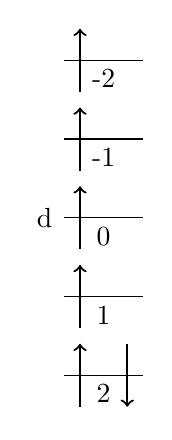
\begin{tikzpicture}
      % d
      \draw (0-0.25,0) circle (0) node {d};
      \draw (0, 2) -- node[below] {-2} (1, 2);
      \draw (0, 1) -- node[below] {-1} (1, 1);
      \draw (0, 0) -- node[below] { 0} (1, 0);
      \draw (0,-1) -- node[below] { 1} (1,-1);
      \draw (0,-2) -- node[below] { 2} (1,-2);
      \draw[->,thick] (0.2, 2-0.4) -- (0.2, 2+0.4);
      \draw[->,thick] (0.2, 1-0.4) -- (0.2, 1+0.4);
      \draw[->,thick] (0.2, 0-0.4) -- (0.2, 0+0.4);
      \draw[->,thick] (0.2,-1-0.4) -- (0.2,-1+0.4);
      \draw[->,thick] (0.2,-2-0.4) -- (0.2,-2+0.4);
      \draw[<-,thick] (0.8,-2-0.4) -- (0.8,-2+0.4);
    \end{tikzpicture}
    \caption{Ground State of Fe}
  \end{figure}
\item Find $L$ by adding up all of the values on the sides for every electron that is present, in the example above, we would have $L=2+2+1+0-1-2=2$. 
\item The term symbol changes depending on $L$, the most common are $S,P,D,F$ for $L=0,1,2,3$ respectively
\item Find $S$ by adding $1/2$ for every up arrow, and adding $-1/2$ for every down arrow. Multiply it by two and add 1 to get the upper left symbol
\item If the shell is half full or more than half full, get the lower right symbol by adding $L$ and $S$, it is less than half full, take the absolute value of their difference. 
\end{enumerate}
\subsection{Solids}
In solids, the valence electrons are free to move, there are two models we will look at, the electron gas and the Bloch model
\subsubsection{The Free Electron Gas}
Suppose we have a rectangular solid, with dimensions $l_x$, $l_y$ and $l_z$, and an electron inside experiences no forces at all except at the walls:
\begin{align*}
  V(x,y,z)=
  \begin{cases}
    0 & 0<x<l_x,0<y<l_y,0<z<l_z\\
    \infty & \text{otherwise}
  \end{cases}
\end{align*}
The Schrodinger equation gives:
\begin{align*}
  -\dfrac{\hbar^2}{2m}\laplacian{\psi}=E\psi
\end{align*}
In Cartesian coordinates we get:
\begin{align*}
  -\dfrac{\hbar^2}{2m}\dv[2]{X}{x}=E_xX\qquad
  -\dfrac{\hbar^2}{2m}\dv[2]{Y}{y}=E_yY\qquad
  -\dfrac{\hbar^2}{2m}\dv[2]{Z}{z}=E_zZ
\end{align*}
Where the total energy is the sum $E_x+E_y+E_z$, Using usual coefficient substitution we have:
\begin{align*}
  k_x\equiv\dfrac{\sqrt{2mE_x}}{\hbar}\qquad
  k_y\equiv\dfrac{\sqrt{2mE_y}}{\hbar}\qquad
  k_z\equiv\dfrac{\sqrt{2mE_z}}{\hbar}
\end{align*}
The first boundary conditions give:
\begin{align*}
  X(x)=A_x\sin(k_xx)\qquad Y(y)=A_y\sin(k_yy)\qquad Z(z)=A_z\sin(k_zz)
\end{align*}
And we get restrictions on the $k$s from the other condition:
\begin{align*}
  k_xl_x=n_x\pi\qquad k_yl_y=n_y\pi\qquad k_zl_z=n_z\pi
\end{align*}
And each of the $n_i$ is a positive integer. Going through the regular infinite square well normalization gives:
\begin{align*}
  \psi_{n_xn_yn_z}=\sqrt{\dfrac{8}{l_xl_yl_z}}
  \sin(\dfrac{n_x\pi}{l_x}x)\sin(\dfrac{n_y\pi}{l_y}y)\sin(\dfrac{n_z\pi}{l_z}z)
\end{align*}
And the energies are:
\begin{align*}
  E_{n_xn_yn_z}=\dfrac{\hbar^2\pi^2}{2m}
  \qty(\dfrac{n_x^2}{l_x^2}+\dfrac{n_y^2}{l_y^2}+\dfrac{n_z^2}{l_z^2})=
  \dfrac{\hbar^2k^2}{2m}
\end{align*}
We now shift to a space where the axes are given by the three $k$ variables, and lines are drawn at $\pi/l_i$. This means each block occupies a space with the volume:
\begin{align*}
  \dfrac{\pi^3}{l_xl_yl_z}=\dfrac{\pi^3}{V}
\end{align*}
But this is not a volume in the traditional sense, it a volume in $k$-space. The solid contains $N$ atoms with $d$ free electrons per atom. If the electrons were distinguishable, or bosons, they would all be in the $\psi_{111}$ state, but alas they are not, due to the Pauli exclusion principle they cannot all occupy $\psi_{111}$ together. These electrons will fill out an octant of a sphere in $k$-space, whose radius is some Fermi wavenumber $k_F$. Since each pair of electrons effectively fills an chunk in $k$-space, we have:
\begin{align*}
  \dfrac{1}{8}\qty(\dfrac{4}{3}\pi k_F^3)=\dfrac{Nd}{2}\qty(\dfrac{\pi^3}{V})
\end{align*}
Solving for $k_F$ results in:
\begin{align*}
  k_F^3=\dfrac{3Nd\pi^2}{V}=3\rho\pi^2
\end{align*}
Where $\rho$ is the free electron density. This Fermi wavenumber defines a Fermi energy given by:
\begin{align*}
  E_F=\dfrac{\hbar^2}{2m}\qty(3\rho\pi^2)^{3/2}
\end{align*}
The total energy of the electron gas can be calculated by finding the volume of a shell with thickness $\dd{k}$:
\begin{align*}
  \dd{V}=\dfrac{1}{8}\qty(4\pi k^2)\dd{k}
\end{align*}
The number of states in the shell is:
\begin{align*}
  \dfrac{2\qty((1/2)\pi k^2\dd{k})}{\pi^3/V}=\dfrac{V}{\pi^2}k^2\dd{k}
\end{align*}
So the differential energy is:
\begin{align*}
  \dd{E}=\dfrac{\hbar^2}{2m}\dfrac{V}{\pi^2}k^2\dd{k}=\dfrac{\hbar^2V}{2\pi^2m}k^4\dd{k}
\end{align*}
So the total energy of filled states is:
\begin{align*}
  E_{tot}=\dfrac{\hbar^2V}{2\pi^2m}\int_0^{k_F}k^4\dd{k}=\dfrac{\hbar^2k_F^5V}{10\pi^2m}=
  \dfrac{\hbar^2(3\pi^2Nd)^{5/3}}{10\pi^2m}V^{-2/3}
\end{align*}
\subsubsection{Band Structure}
We start this section by defining a periodic potential, such that:
\begin{align*}
  V(x+a)=V(x)
\end{align*}
Bloch's theorem says that the such potentials satisfy the Schrodinger equation with an additional boundary condition:
\begin{align*}
  \psi(x+a)=\exp{iqa}\psi(x)
\end{align*}
The constant $q$ is independent of position, it may however depend on other factors. It is important to note that this additional phase does not change the normalization:
\begin{align*}
  \abs{\psi(x+a)}^2=\abs{\psi(x)}^2
\end{align*}
Now, no real solid goes on forever, so we can just wrap the $x$ axis around after some point $N$:
\begin{align*}
  \psi(x+Na)=\psi(x)
\end{align*}
So we get that:
\begin{align*}
  \exp{iNqa}\psi(x)=\psi(x)
\end{align*}
So we have that:
\begin{align*}
  \exp{iNqa}=1\implies Nqa=2\pi n
\end{align*}
And the values of $q$ are:
\begin{align*}
  q=\dfrac{2\pi n}{Na}
\end{align*}
Where $n =0,\pm1,\pm2...$. One potential we can consider is the Dirac comb:
\begin{align*}
  V(x)=\alpha\sum_{j=0}^{N-1}\delta(x-ja)
\end{align*}
We solve the Schrodinger equation in the region between delta functions:
\begin{align*}
  \dv[2]{\psi}{x}=-\dfrac{2mE}{\hbar^2}\psi=-k^2\psi
\end{align*}
Which has the general solution of:
\begin{align*}
  \psi(x)=A\sin(kx)+B\cos(kx)
\end{align*}
Invoking Bloch's theorem, the wavefunction immediately left of the origin is:
\begin{align*}
  \psi(x)=\exp{-iqa}\qty(A\sin(k(x+a))+B\cos(k(x+a)))
\end{align*}
The wavefunction must be continuous at $x=0$, so we get:
\begin{align*}
  B=\exp{-iqa}\qty[A\sin(ka)+B\cos(ka)]
\end{align*}
The derivative inherits the discontinuity as well, so we get from previous quantities:
\begin{align*}
  kA-\exp{-iqa}k\qty(A\cos(ka)-B\sin(ka))=\dfrac{2m\alpha}{\hbar^2}B
\end{align*}
We can solve for $A\sin(ka)$:
\begin{align*}
  A\sin(ka)=\qty[\exp{iqa}-\cos(ka)]B
\end{align*}
Using the other equation, we can find that:
\begin{align*}
  \qty[\exp{iqa}-\cos(ka)]\qty[1-\exp{-iqa}\cos(ka)]+\exp{-iqa}\sin^2(ka)=
  \dfrac{2m\alpha}{\hbar^2k}\sin(ka)
\end{align*}
This can simplify to:
\begin{align*}
  \cos(qa)=\cos(ka)+\dfrac{m\alpha}{\hbar^2k}\sin(ka)
\end{align*}
This is a transcendental equation, we define $z\equiv ka$ and $\beta\equiv m\alpha a/\hbar^2$. Giving the right side as:
\begin{align*}
  f(z)\equiv\cos(z)+\beta\dfrac{\sin(z)}{z}
\end{align*}
Where we can find intersections with $\pm1$ since $\cos(qa)$ is going to be one of those. 

% -*- TeX-master: "master.tex" -*-
\section{Symmetries \& Conservation Laws}
\subsection{The Translation Operator}
We define the action of the translation operator by its action on a wavefunction:
\begin{align*}
  \hat{T}(a)\psi(x)=\psi(x-a)
\end{align*}
We can replace $\psi(x-a)$ with its Taylor series:
\begin{align*}
  \psi(x-a)=\sum_n\dfrac{(-a)^n}{n!}\dv[n]{x}\psi(x)
\end{align*}
The argument acting on the wavefunction acts like the momentum operator:
\begin{align*}
  \hat{T}(a)\psi(x)=\sum_n\dfrac{1}{n!}\qty(\dfrac{-ia}{\hbar}\hat{p})^n\psi(x)
\end{align*}
This is the exponential of an operator:
\begin{align*}
  \hat{T}(a)=\mathrm{exp}\qty[-\dfrac{ia}{\hbar}\hat{p}]
\end{align*}
This means that momentum is the generator for translations. The translation operator is a unitary operator:
\begin{align*}
  \hat{T}(a)^{-1}=\hat{T}(-a)=\hat{T}(a)^\dag
\end{align*}
\subsubsection{Transforming Operators}
Translating an operator $\hat{Q}$ to an operator $\hat{Q}'$ gives:
\begin{align*}
  \hat{Q}'=\hat{T}^\dag\hat{Q}\hat{T}
\end{align*}
\subsubsection{Translational Symmetry}
A system is translationally invariant if the Hamiltonian is unchanged by translation, that is:
\begin{align*}
  \hat{H}'=\hat{T}^\dag\hat{H}\hat{T}=\hat{H}
\end{align*}
However, because $\hat{T}$ is unitary, we can say:
\begin{align*}
  \hat{H}\hat{T}=\hat{T}\hat{H}
\end{align*}
Which means that the commutator is $0$:
\begin{align*}
  \comm{\hat{H}}{\hat{T}}=0
\end{align*}
The one dimensional Hamiltonian for a particle of mass $m$:
\begin{align*}
  \hat{H}=\dfrac{\hat{p}^2}{2m}+V(x)
\end{align*}
The translated operator is:
\begin{align*}
  \hat{H}'=\dfrac{\hat{p}^2}{2m}+V(x+a)
\end{align*}
Translational symmetry must imply that:
\begin{align*}
  V(x+a)=V(x)
\end{align*}
This is like the Dirac comb! For continuous translational symmetries, we consider infinitesimal translations $\delta$:
\begin{align*}
  \hat{T}(\delta)=\exp{-i\delta\hat{p}/\hbar}\approx 1-i\dfrac{\delta}{\hbar}\hat{p}
\end{align*}
The commutator with the Hamiltonian is:
\begin{align*}
  \comm{\hat{H}}{\hat{T}(\delta)}=\comm{\hat{H}}{1-i\dfrac{\delta}{\hbar}\hat{p}}=0
  \implies\comm{\hat{H}}{\hat{p}}=0
\end{align*}
From this, the generalized Ehrenfest theorem will tell us that:
\begin{align*}
  \dv{t}\ev{p}=0
\end{align*}
So momentum conservation comes from continuous translational symmetries. This is an instance of Noether's theorem. 
\subsection{Conservation Laws}
We want to talk about what it means for a quantity to be conserved. It includes the following two concepts:
\begin{enumerate}
\item The expectation value is independent of time.
\item The probability of getting any particular value is independent of time. 
\end{enumerate}
The first condition means that the operator must commute with the Hamiltonian. The same criterion guarantees conservation by the second definition as well. 
\subsection{Parity}
\subsubsection{Parity in One Dimension}
We define the parity operator in one dimension as:
\begin{align*}
  \hat{\Pi}\psi(x)=\psi'(x)=\psi(-x)
\end{align*}
The parity operator is its own inverse and it is self adjoint. Altogether, the operator is unitary:
\begin{align*}
  \hat{\Pi}^{-1}=\hat{\Pi}=\hat{\Pi}^\dag
\end{align*}
Transforming an operator becomes:
\begin{align*}
  \hat{Q}'=\hat{\Pi}^\dag\hat{Q}\hat{\Pi}
\end{align*}
Position and momentum are odd under parity:
\begin{align*}
  \hat{x}'=\hat{\Pi}^\dag\hat{x}\hat{\Pi}=-\hat{x}
  \hat{p}'=\hat{\Pi}^\dag\hat{p}\hat{\Pi}=-\hat{p}
\end{align*}
Transforming a general operator:
\begin{align*}
  \hat{Q}'(\hat{x},\hat{p})=\hat{Q}(-\hat{x},-\hat{p})
\end{align*}
A system with inversion symmetry has the Hamiltonian commuting with the parity operator:
\begin{align*}
  \comm{\hat{H}}{\hat{\Pi}}=0
\end{align*}
The potential must be an even function of position:
\begin{align*}
  V(x)=V(-x)
\end{align*}
This means that parity is conserved with time, so if a wavefunction at one point of time is even, it will stay even. In the same vein, if it is odd it will stay odd. An example is the harmonic oscillator potential. 
\subsubsection{Parity in Three Dimensions}
In $3-D$ the parity operator is given by:
\begin{align*}
  \hat{\Pi}\psi(\vb{r})=\psi'(\vb{r})=\psi(-\vb{r})
\end{align*}
The $3-D$ momentum and position operators transform the same. Again the potential must be even:
\begin{align*}
  V(\vb{r})=V(-\vb{r})
\end{align*}
The eigenstates of a particle in a central potential are also eigenstates of parity:
\begin{align*}
  \hat{\Pi}\psi_{n\ell m}=(-1)^\ell\psi_{n\ell m}
\end{align*}
\subsection{Rotational Symmetry}
\subsubsection{Rotations About the z Axis}
The operator that rotates a function about the $z$ axis by an angle $\phi$ is $\hat{R}_z$:
\begin{align*}
  \hat{R}_z(\varphi)\psi(r,\theta,\phi)=\psi'(r,\theta,\phi)=\psi(r,\theta,\phi+\varphi)
\end{align*}
It turns out that angular momentum is the generator of rotations:
\begin{align*}
  \hat{R}_z(\varphi)=\mathrm{exp}\qty[-\dfrac{i\varphi}{\hbar}\hat{L}_z]
\end{align*}
For an infinitesimal angle $\delta$:
\begin{align*}
  \hat{R}_z(\delta)\approx -\dfrac{i\delta}{\hbar}\hat{L}_z
\end{align*}
Finding the transformed operators allows us to find the matrix form:
\begin{align*}
  \pmqty{\hat{x}'\\\hat{y}'\\\hat{z}'}=
  \pmqty{1&-\delta&0\\\delta&1&0\\0&0&1}\pmqty{\hat{x}\\\hat{y}\\\hat{z}}
\end{align*}
This is a truncated Taylor series of a normal rotation matrix.
\subsubsection{Rotations in Three Dimensions}
Rotation about an arbitrary unit vector $\vb{n}$:
\begin{align*}
  \hat{R}_{\vb{n}}=\mathrm{exp}\qty[-\dfrac{i\varphi}{\hbar}\vb{n}\vdot\hat{\vb{L}}]
\end{align*}
Any vector quantity has the following commutator rule:
\begin{align*}
  \comm{\hat{L}_i}{\hat{V}_j}=i\hbar\epsilon_{ijk}\hat{V}_k
\end{align*}
An example of this is $\hat{\vb{r}}$, $ \hat{\vb{p}}$ and $\hat{\vb{L}}$. A scalar operator is invariant under rotation:
\begin{align*}
  \comm{\hat{L}_i}{\hat{f}}=0
\end{align*}
We have the following table for various quantities:
\begin{table}[H]
\centering
\begin{tabular}{ccc}
\hline
 & Parity & Rotations \\ \hline
True Vector $\hat{\vb{V}}$ & $\acomm{\hat{\Pi}}{\hat{V}_i}=0$ & $\comm{\hat{\L}_i}{\hat{V}_j}=i\hbar\epsilon_{ijk}\hat{V}_k$ \\
Pseudovector $\hat{\vb{V}}$ & $\comm{\hat{\Pi}}{\hat{V}_i}=0$ & $\comm{\hat{\L}_i}{\hat{V}_j}=i\hbar\epsilon_{ijk}\hat{V}_k$ \\
True Scalar $\hat{f}$ & $\comm{\hat{\Pi}}{\hat{f}}=0$ & $\comm{\hat{\L}_i}{\hat{f}}=0$ \\
Pseudoscalar $\hat{f}$ & $\acomm{\hat{\Pi}}{\hat{f}}=0$ & $\comm{\hat{\L}_i}{\hat{f}}=0$ \\ \hline
\end{tabular}
\end{table}
For infinitesimal rotations we get:
\begin{align*}
  \hat{R}_{\vb{n}}(\delta)\approx 1-\dfrac{i\delta}{\hbar}\vb{n}\vdot\hat{\vb{L}}
\end{align*}
Hence the Hamiltonian commutes with the three components of angular momentum. Which leads to angular momentum conservation. 
\subsection{Degeneracy}
We know that the existence of a symmetry means there is an operator $\hat{Q}$ that commutes with the Hamiltonian:
\begin{align*}
  \comm{\hat{H}}{\hat{Q}}=0
\end{align*}
The basic idea of it is that given a stationary state $\ket{\psi_n}$, then $\hat{Q}\ket{\psi_n}$ is a stationary state with the same energy. The proof goes like:
\begin{align*}
  \hat{H}\ket{\psi_n'}=\hat{H}\qty(\hat{Q}\ket{\psi_n})=
  \hat{Q}\hat{H}\ket{\psi_n}=\hat{Q}E_n\ket{\psi_n}=E_n\qty(\hat{Q}\psi{n})=
  E_n\ket{\psi_n'}
\end{align*}
However, this is not always true, since the state and transformed state might be the same. 
\subsection{Rotational Selection Rules}
\subsubsection{Scalar Quantities}
The selection rules for rotation with a scalar operator can be written as:
\begin{align*}
  \mel{n'\ell'm'}{\hat{f}}{n\ell m}=
  \delta_{\ell\ell'}\delta_{mm'}\mel{n'\ell|}{\hat{f}}{|n\ell}
\end{align*}
\subsubsection{Vector Quantities}
We can define a general raising and lowering operator as:
\begin{align*}
  \hat{V}_\pm\equiv\hat{V}_x\pm i\hat{V}_y
\end{align*}
The selection rules of $m$ are:
\begin{align*}
  \mel{n'\ell'm'}{\hat{V}_+}{n\ell m}=0\quad&\quad\text{unless $m'=m+1$}\\
  \mel{n'\ell'm'}{\hat{V}_z}{n\ell m}=0\quad&\quad\text{unless $m'=m$}\\
  \mel{n'\ell'm'}{\hat{V}_-}{n\ell m}=0\quad&\quad\text{unless $m'=m-1$}
\end{align*}
Turning this into the $x$ and $y$ components can be gotten from:
\begin{align*}
  \mel{n'\ell'm'}{\hat{V}_x}{n\ell m}&=\dfrac{1}{2}
  \qty[\mel{n'\ell'm'}{\hat{V}_-}{n\ell m}+\mel{n'\ell'm'}{\hat{V}_+}{n\ell m}]\\
  \mel{n'\ell'm'}{\hat{V}_y}{n\ell m}&=\dfrac{i}{2}
  \qty[\mel{n'\ell'm'}{\hat{V}_-}{n\ell m}-\mel{n'\ell'm'}{\hat{V}_+}{n\ell m}]
\end{align*}
The selection rules for $\ell$ can be summarized by:
\begin{align*}
  \mel{n'\ell'm'}{\hat{V}_+}{n\ell m}&=
  -\sqrt{2}C_{m1m'}^{\ell1\ell'}\mel{n\ell'|}{V}{|n\ell}\\
  \mel{n'\ell'm'}{\hat{V}_-}{n\ell m}&=
  \sqrt{2}C_{m-1m'}^{\ell1\ell'}\mel{n\ell'|}{V}{|n\ell}\\
  \mel{n'\ell'm'}{\hat{V}_z}{n\ell m}&=C_{m0m'}^{\ell1\ell'}\mel{n\ell'|}{V}{|n\ell}
\end{align*}
These all require the $m$ and $\ell$ values satisfy the following:
\begin{align*}
  \ell-\ell'=\pm1\quad\text{and}\quad m-m'=\pm1
\end{align*}
\subsection{Translations in Time}
We define the time translation operator as:
\begin{align*}
  \hat{U}\Psi(x,0)=\Psi(x,t)
\end{align*}
Doing the same procedure as before, we can find that:
\begin{align*}
  \hat{U}(t)=\mathrm{exp}\qty[-\dfrac{it}{\hbar}\hat{H}]
\end{align*}
We define the Heisenberg equivalent of a Schrodinger picture operator as:
\begin{align*}
  \hat{Q}_H(t)=\hat{U}^\dag(t)\hat{Q}\hat{U}(t)
\end{align*}
Where the Hermitian conjugate of $\hat{U}$ is given by:
\begin{align*}
  \hat{U}^\dag(t)=\mathrm{exp}\qty[\dfrac{it}{\hbar}\hat{H}]
\end{align*}
It turns out that time translation invariance leads to energy conservation.
% -*- TeX-master: "master.tex" -*-
\section{Time Independent Perturbation Theory}
The fundamental idea behind the time independent perturbation is that we are trying to solve the Schrodinger equation for a potential that is equivalent to a potential we know how to solve plus a little dip, called a perturbation. This can be expressed as:
\begin{align*}
H=H^0+H'
\end{align*}
Where $H^0$ represents the solvable Hamiltonian, and $H'$ is the perturbation. We know for sure that the unperturbed Hamiltonian ($H'=0$) can be solved with the following eigenfunctions:
\begin{align*}
  H^0\psi_n^0=E_n^0\psi_n^0
\end{align*}
These eigenfunctions are orthogonal and normalized:
\begin{align*}
  \ip{\psi_n^0}{\psi_m^0}=\delta_{m,n}
\end{align*}
\subsection{Non-Degenerate Perturbation Theory}
Our overall goal is to solve the Schrodinger equation:
\begin{align*}
  H\psi_n=E_n\psi_n
\end{align*}
For perturbed energies and eigenfunctions. We can estimate the full Hamiltonian with a parameter $\lambda$:
\begin{align*}
  H=H^0+\lambda H'
\end{align*}
Then we expand each of the eigenvalues and eigenfunctions in powers of lambda, where the superscript will denote the order of correction:
\begin{align*}
  \psi_n&=\psi_n^0+\lambda\psi_n^1+\lambda^2\psi_n^2+\cdots\\
  E_n&=E_n^0+\lambda E_n^1+\lambda^2E_n^2+\cdots
\end{align*}
Replacing the Hamiltonian and the eigenfunctions with these expansions:
\begin{align*}
  \qty(H^0+\lambda H')\qty[\psi_n^0+\lambda\psi_n^1+\lambda^2\psi_n^2]=
  \qty(E_n^0+\lambda E_n^1+\lambda^2E_n^2)\qty[\lambda\psi_n^1+\lambda^2\psi_n^2]
\end{align*}
Lets collect like powers of $\lambda$:
\begin{align*}
  &H^0\psi_n^0+\lambda\qty(H^0\psi_n^1+H'\psi_n^0)+\lambda^2\qty(H^0\psi_n^2+H'\psi_n^1)\\
  &=E_n^0\psi_n^0+\lambda\qty(E_n^0\psi_n^1+E_n^1\psi_n^0)+
  \lambda^2\qty(E_n^0\psi_n^2+E_n^1\psi_n^1+E_n^2\psi_n^0)
\end{align*}
From the definition of the 0th order terms, the constant terms are ignored, since its the unperturbed eigenvalue problem, so they can be subtracted. This is a polynomial, so in order to achieve equality we need to match like powers of $\lambda$:
\begin{align*}
  \lambda&:\quad H^0\psi_n^1+H'\psi_n^0=E_n^0\psi_n^1+E_n^1\psi_n^0\\
  \lambda^2&:\quad H^0\psi_n^2+H'\psi_n^1=E_n^0\psi_n^2+E_n^1\psi_n^1+E_n^2\psi_n^0
\end{align*}
\subsubsection{First Order Corrections}
We start by completing the first order term with an inner product with $\psi_n^0$:
\begin{align*}
  \ip{\psi_n^0}{H^0\psi_n^1}+\ip{\psi_n^0}{H'\psi_n^0}=
  E_n^0\ip{\psi_n^0}{\psi_n^1}+E_n^1\ip{\psi_n^0}{\psi_n^0}
\end{align*}
However, since $H^0$ (not necessarily $H'$) is Hermitian, we can move it into the bra so that it acts on an eigenfunction, so we end up with:
\begin{align*}
  \ip{\psi_n^0}{H^0\psi_n^1}=\ip{H^0\psi_n^0}{\psi_n^1}=\ip{E_n^0\psi_n^0}{\psi_n^1}=
  E_n^0\ip{\psi_n^0}{\psi_n^1}
\end{align*}
The term with the two non-corrected eigenfunctions just goes away since we have normalized eigenfunctions. All of this combined will give us:
\begin{align*}
  E_n^0\ip{\psi_n^0}{\psi_n^1}+\ip{\psi_n^0}{H'\psi_n^0}&=
  E_n^0\ip{\psi_n^0}{\psi_n^1}+E_n^1\\
  \ip{\psi_n^0}{H'\psi_n^0}&=E_n^1
\end{align*}
Hence the first order correction term for the energy is:
\begin{align*}
  \boxed{E_n^1=\mel{\psi_n^0}{H'}{\psi_n^0}}
\end{align*}
If we take the first order $\lambda$ terms again, we get:
\begin{align*}
  \qty(H^0-E_n^0)\psi_n^1=-\qty(H'-E_n^1)\psi_n^0
\end{align*}
The first order correction to the wavefunction must be a well-behaved function, and since the solutions to the unperturbed Hamiltonian form a complete set, we can write the first order correction in terms of them:
\begin{align*}
  \psi_n^1=\sum_{m\neq n}c_m^{(n)}\psi_m^0
\end{align*}
We don't include the $n^{th}$ term since it is included above. Using the relation above, we get:
\begin{align*}
  \sum_{m\neq n}\qty(E_m^0-E_n^0)c_m^{(n)}\psi_m^0=-\qty(H'-E_n^1)\psi_n^0
\end{align*}
Take an inner product with $\psi_l^0$:
\begin{align*}
  \sum_{m\neq n}\qty(E_m^0-E_n^0)c_m^{(n)}\ip{\psi_l^0}{\psi_m^0}=
  -\qty(H'-E_n^1)\ip{\psi_l^0}{\psi_n^0}
\end{align*}
Hence the constant is given by:
\begin{align*}
  c_m^{(n)}=\frac{\mel{\psi_m^0}{H'}{\psi_n^0}}{E_n^0-E_m^0}
\end{align*}
Hence the first order correction to the wavefunction:
\begin{align*}
  \psi_n^1=\sum_{m\neq n}\frac{\mel{\psi_m^0}{H'}{\psi_n^0}}{E_n^0-E_m^0}\psi_m^0
\end{align*}
You will notice that the denominator is $0$ if the energies are equal, hence if there are degenerate energies. For this we need degenerate perturbation theory.
\subsubsection{Second Order Correction}
Taking an inner product as we did before with the second order lambda term this time, we get:
\begin{align*}
  \ip{\psi_n^0}{H^0\psi_n^2}+\ip{\psi_n^0}{H'\psi_n^1}=
  E_n^0\ip{\psi_n^0}{\psi_n^2}+E_n^2\ip{\psi_n^0}{\psi_n^0}
\end{align*}
After applying the same tricks, we end up with:
\begin{align*}
  E_n^2=\mel{\psi_n^0}{H'}{\psi_n^1}-E_n^1\ip{\psi_n^0}{\psi_n^1}
\end{align*}
But the second term is 0, hence we can simplify this to:
\begin{align*}
  E_n^2=\sum_{m\neq n}\frac{\abs{\mel{\psi_m^0}{H'}{\psi_n^0}}^2}{E_n^0-E_n^0}
\end{align*}
\subsection{Degenerate Perturbation Theory}
States are degenerate if their wavefunctions are different, but their energies are the same. Lets go through an example of two-fold degeneracy.
\subsubsection{Two-Fold}
This example of degeneracy has two states which are orthogonal, $\psi_a,\psi_b$, but both with the same energy:
\begin{align*}
  H^0\psi_a^0=E^0\psi_a^0\quad H^0\psi_b^0=E^0\psi_b^0\quad\ip{\psi_a}{\psi_b}=0
\end{align*}
Any linear combination of the states are also an eigenstate of the unperturbed Hamiltonian with the same energy.

To find the coefficients, we need to diagonalize the $W$ matrix, whose elements are given by:
\begin{align*}
  W_{ij}=\mel{\psi_i^0}{H'}{\psi_j^0}
\end{align*}
So the total eigenvalue problem would be:
\begin{align*}
  \pmqty{W_{aa}&W_{ab}\\W_{ba}&W_{bb}}\pmqty{\alpha\\\beta}=E^1\pmqty{\alpha\\\beta}
\end{align*}
We also have a theorem:

Let $A$ be a hermitian operator that commutes with $H^0$ and $H'$. If $\psi_a^0$ and $\psi_b^0$ are also eigenfunctions of A, with distinct eigenvalues:
\begin{align*}
  A\psi_a^0=\mu\psi_a^0\quad A\psi_b^0=\nu\psi_b^0
\end{align*}
Such that $\mu\neq\nu$. Then, $\psi_a^0$ and $\psi_b^0$ are the good states to use in perturbation theory. We can prove this but I do not want to.
\subsubsection{Higher Order}
To conquer higher order degeneracies, you simply need to grow your $W$ matrix
% -*- TeX-master: "master.tex" -*-
\section{The Variational Principle}
The variational principle states that:
\begin{align*}
  E_{gs}\leq\ev{H}=\mel{\psi}{H}{\psi}
\end{align*}
Where $\psi$ is any normalized function.
The process for the variational method is very simple, and follows these steps:
\begin{enumerate}
\item Find a wavefunction that matches the potential with a parameter that can be varied. For example it could be the Gaussian:
  \begin{align*}
    \psi = A\exp{-bx^2}
  \end{align*}
Which matches very well with potentials that do not have barriers. 
\item Normalize the function, it will usually be in terms of the parameter that you built in.
\item Find the expectation value of the Hamiltonian, which can be written in terms of the kinetic and potential energy:
  \begin{align*}
    \ev{H}&=\ev{T}+\ev{V}\\
    \ev{T}&=\ev{-\frac{\hbar^2}{2m}\laplacian}\\
    \ev{V}&=\ev{V}
  \end{align*}
  Where $V$ is the potential for the specific problem.
\item Minimize the Hamiltonian with respect to the parameter:
  \begin{align*}
    \ev{H}_{min}=E_{gs}\implies \pdv{\ev{H}}{b}=0
  \end{align*}
  If you have multiple parameters you can minimize with respect to all of them
\item The previous result should give a value for the parameter, plug that into the Hamiltonian, and you should get a result without any of the parameters. This results in the estimation for the ground state. 
\end{enumerate}
% -*- TeX-master: "master.tex" -*-
\section{The WKB Approximation}
The essential idea of the WKB method is to find energies in regions of constant potential. For a particle with energy greater than the potential, we know that the wavefunction will look like:
\begin{align*}
  \psi(x)=A\exp{\pm ikx}\quad k=\sqrt{2m(E-V)}/\hbar
\end{align*}
Where, just like in the initial scattering section, $\pm$ corresponds to a particle travelling to the right or left respectively. If $E<V$ we have $\kappa$ instead:
\begin{align*}
  \psi(x)=A\exp{\pm \kappa x}\quad \kappa=\sqrt{2m(V-E)}/\hbar
\end{align*}
If $V(x)$ is not constant, but rather varies slowly with respect to some parameter, we know that the solutions will be practically exponential/sinusoidal. 

The one region where these dont work are when $E\approx V$ where $\kappa$ or $k$ go to $0$. These regions are called classical turning points. We should ignore these first.
\subsection{The "Classical" Region}
The classical region is where a particle would be confined to in classical mechanics, where $E\geq V(x)$.

We can rewrite the (time dependent) Schrodinger equation in terms of the classical momentum $p$:
\begin{align*}
  \dv[2]{\psi}{x}=-\frac{p^2}{\hbar^2}\psi
\end{align*}
With the classical momentum now written as:
\begin{align*}
  p(x)\equiv\sqrt{2m(E-V(x))}
\end{align*}
Now, instead of writing the solution with constant amplitude and phase, we rewrite them as functions of position since they wont be constant, but rather slowly varying:
\begin{align*}
  \psi(x)=A(x)\exp{i\phi(x)}
\end{align*}
We can plug this into the Schrodinger equation again to find equations for $A$ and $\phi$ in terms of $V$:
\begin{align*}
  A''&=A\qty[(\phi')^2-\frac{p^2}{\hbar^2}]\\
  \qty(A^2\phi')'&=0
\end{align*}
The second equation can immediately be solved:
\begin{align*}
  A=\frac{C}{\sqrt{\abs{\phi'}}}
\end{align*}
Plugging this into the other one gives us an immediate solution of:
\begin{align*}
  \phi(x)=\pm\frac{1}{\hbar}\int p(x)\dd{x}
\end{align*}
Hence the wavefunction can be written as:
\begin{align*}
  \psi(x)=\frac{C}{\sqrt{p(x)}}\exp{\pm\frac{i}{\hbar}\int p(x)\dd{x}}
\end{align*}
For a potential well with two vertial walls, we end up with the following that leads to the energies:
\begin{align*}
  \int_0^ap(x)\dd{x}=n\pi\hbar
\end{align*}
This is for potentials of the form:
\begin{align*}
  V(x)=
  \begin{cases}
    \text{some function} & 0<x<a\\
    \inf & \text{otherwise}
  \end{cases}
\end{align*}
Or something similar
\subsection{Tunneling}
In non-classical regions, the classical momentum can be imaginary, so if we have a tunneling problem where $E<V$, we have:
\begin{align*}
  \psi(x)\approx\frac{C}{\sqrt{\abs{p(x)}}}\exp{\pm\frac{1}{\hbar}\int\abs{p(x)}\dd{x}}
\end{align*}
In the case of a rectangular barrier with a curvy top, we end up with the following transmission coefficient:
\begin{align*}
  T&=\exp{-2\gamma}\\
  \gamma&\equiv\frac{1}{\hbar}\int_0^a\abs{p(x)}\dd{x}
\end{align*}
\subsection{Connection Formulas}
We are dealing with turning points now, such that $E=V$. For simplicity lets move the axes such that the turning point occurs at $x=0$:
\begin{align*}
  \psi(x)\approx
  \begin{cases}
    \qty[B\exp{i\int_x^0p(x')\dd{x'}/\hbar}+C\exp{-i\int_x^0p(x')\dd{x'}/\hbar}]/
    \sqrt{p(x)}
    & x < 0 \\
    D\exp{-\int_0^x\abs{p(x')}\dd{x'}/\hbar}/\sqrt{\abs{p(x)}}
    & x > 0
  \end{cases}
\end{align*}
The problem is that the momentum goes to $0$ at the turning points, so $\psi\to\infty$. The solution is to use a patching function that covers the turning point and a patching region. We do this by linearizing the potential in this neighborhood:
\begin{align*}
  V(x)\approx E+V'(0)x
\end{align*}
And then solve the Schrodinger equation for the linearized potential:
\begin{align*}
  -\frac{\hbar^2}{2m}\dv[2]{\psi_p}{x}+(E+V'(0)x)\psi_p=E\psi_p
\end{align*}
We end up with the Airy's differential equation:
\begin{align*}
  \dv[2]{\psi_p}{z}=z\psi_p
\end{align*}
This leads to the following equation for $\psi(x)$, with one normalization constant and shifting the turning point:
\begin{align*}
  \psi(x)=
  \begin{cases}
    2D/\sqrt{p(x)}\sin\int_x^{x_2}p(x')\dd{x'}/\hbar & x < x_2 \\
    D/\sqrt{\abs{p(x)}}\exp{-\int_x^{x_2}\abs{p(x')}\dd{x'}/\hbar} & x > x_2
  \end{cases}
\end{align*}
If we have a downward sloping turning point, we get:
\begin{align*}
  \psi(x)=
  \begin{cases}
    D'/\sqrt{\abs{p(x)}}\exp{-\int_x^{x_1}\abs{p(x')}\dd{x'}/\hbar} & x < x_1\\
    2D'/\sqrt{p(x)}\sin\int_x^{x_2}p(x')\dd{x'}/\hbar & x > x_1
  \end{cases}
\end{align*}
If a potential well has one vertical wall and one sloping wall (turning point), we can find the energies by integrating the momentum:
\begin{align*}
  \int_0^{x_2}p(x)\dd{x}=\qty(n-\frac{1}{4})\pi\hbar
\end{align*}
To find the energies of a potential with no vertical walls, we use the following:
\begin{align*}
  \int_{x_1}^{x_2}p(x)\dd{x}=\qty(n-\frac{1}{2})\pi\hbar
\end{align*}
In all of these cases, $n$ runs from $1$ on to infinity, not $0$.
% -*- TeX-master: "master.tex" -*-
\section{Scattering}
Important formulas for Scattering:
\subsection{Classical Scattering}
Definition of $\dd{\sigma}$ and $\sigma$
\begin{align*}
  \dd{\sigma}&=D(\theta)\dd{\Omega}\\
  \sigma&\equiv\int D(\theta)\dd{\Omega}
\end{align*}
\subsection{Quantum Scattering}
We imagine an incoming plane wave, and an outgoing spherical wave, with other stuff happening in the between areas, this wavefunction, for large $r$ looks like:
\begin{align*}
  \psi(r,\theta)\approx A\qty[\exp{ikz}+f(\theta)\frac{\exp{ikr}}{r}]
\end{align*}
Where $k$ has the usual definition:
\begin{align*}
  k\equiv\frac{2mE}{\hbar}
\end{align*}
The differential cross section is related to the $f(\theta)$, called the scattering amplitude:
\begin{align*}
  D(\theta)=\abs{f(\theta)}^2
\end{align*}
So that the differential scattering cross section is:
\begin{align*}
  \sigma=\int\abs{f(\theta)}^2\dd{\Omega}
\end{align*}
\subsection{Partial Waves}
You can solve the Schrodinger equaion to exactly get the form of the wavefunction, in a region where $V(r)=0$:
\begin{align*}
  \psi(r,\theta,\phi)=A\qty[\exp{ikz}+\sum_{\ell,m}C_{\ell,m}h_{\ell}^{(1)}(kr)
    Y_\ell^m(\theta,\phi)]
\end{align*}
Where the only new concept are the spherical hankel functions of the first and second kind $h_\ell^{(1)}$, which are defined as:
\begin{align*}
  h_\ell^{(1)}(x)\equiv j_{\ell}(x)+i n_{\ell}(x)\qquad
  h_\ell^{(2)}(x)\equiv j_{\ell}(x)-i n_{\ell}(x)
\end{align*}
If we take a limit as $r\to\infty$, the hankel function looks like a spherical wave, and we can write the scattering amplitude as:
\begin{align*}
  f(\theta)=\sum_{\ell=0}^\infty\sum_{\ell=0}^{\infty}(2\ell+1)a_\ell P_\ell(\cos\theta)
\end{align*}
Where $a_\ell$ are so called the partial wave amplitudes. The differential and total cross section is given by:
\begin{align*}
  D(\theta)&=\sum_{\ell,\ell'}(2\ell+1)(2\ell'+1)
  a^*_{\ell}a_{\ell'}P_\ell\cos\theta P_{\ell'}\cos\theta\\
  \sigma&=4\pi\sum_{\ell}(2\ell+1)\abs{a_\ell}^2
\end{align*}
\subsection{Phase Shifts}
When we had line scattering we would have a incident and reflected wave, but this phase difference can be generalized:
\begin{align*}
  \psi(x)&=A\qty(\exp{ikx}-\exp{-ikx})\\
  \psi(x)&=A\qty(\exp{ikx}-\exp{i(2\delta-kx)})
\end{align*}
The generic form of these phase shifts can be expressed as:
\begin{align*}
  a_\ell=\frac{1}{k}\exp{i\delta_\ell}\sin\delta_\ell
\end{align*}
So that the scattering amplitude is:
\begin{align*}
  f(\theta)=\frac{1}{k}\sum_{\ell}(2\ell+1)\exp{i\delta_\ell}\sin\delta_\ell P_\ell\cos\theta
\end{align*}
And $\sigma$ is:
\begin{align*}
  \sigma=\frac{4\pi}{k^2}\sum_\ell(2\ell+1)\sin^2\delta_\ell
\end{align*}
\subsection{The Born Approximation}
We can write the Schrodinger equation as an integral using Green's functions:
\begin{align*}
  \qty(\laplacian+k^2)\psi=Q
\end{align*}
Where the quantities are:
\begin{align*}
  k\equiv\frac{\sqrt{2mE}}{\hbar}\qquad Q\equiv\frac{2mV}{\hbar^2}\psi
\end{align*}
The Green's function comes in when we solve for a delta function source:
\begin{align*}
  \qty(\laplacian+k^2)G(\vb{r})=\delta^3(\vb{r})
\end{align*}
Then the wavefunction is expressed as:
\begin{align*}
  \psi(\vb{r})=\int G(\vb{r}-\vb{r}_0Q(\vb{r}_0\dd[3]{\vb{r}_0}
\end{align*}
After some trickery with complex analysis and fourier transforms, we end up with:
\begin{align*}
  \psi(\vb{r})=\psi_0(\vb{r})-\frac{m}{2\pi\hbar^2}
  \int\frac{\exp{ik\abs{\vb{r}-\vb{r}_0}}}{\abs{\vb{r}-\vb{r}_0}}
  V(\vb{r}_0)\psi(\vb{r}_0)\dd[3]{\vb{r}_0}  
\end{align*}
The quantity $\psi_0$ must obey the free particle Schrodinger equation:
\begin{align*}
  \qty(\laplacian+k^2)\psi_0=0
\end{align*}
\subsubsection{First Born Approximation}
We can rewrite the absolute value quantity in fairly simple terms:
\begin{align*}
  \abs{\vb{r-r}_0^2}^2=r^2-r_0^2-2\vb{r\vdot r}_0\approx
  r^2\qty(1-2\frac{\vb{r\vdot r}_0}{r^2})
\end{align*}
Which can be approximated to:
\begin{align*}
  \abs{\vb{r-r}_0^2}\approx r-\vu{r}\vdot\vb{r}_0
\end{align*}
If we define a $k$ vector to be in the $\vu{r}$ direction, we get:
\begin{align*}
  \frac{\exp{ik\abs{\vb{r}-\vb{r}_0}}}{\abs{\vb{r}-\vb{r}_0}}\approx\frac{\exp{ikr}}{r}
  \exp{-i\vb{k}\vdot\vb{r}_0}
\end{align*}
We know for scattering we want $\psi_0$ to be a plane wave, then the wavefunction becomes:
\begin{align*}
  \psi(\vb{r})=A\exp{ikz}-\frac{m}{2\pi\hbar^2}\frac{\exp{ikr}}{r}
  \int\exp{-i\vb{k}\vdot\vb{r}_0}V(\vb{r}_0)\psi(\vb{r}_0)\dd[3]{\vb{r}_0}
\end{align*}
Now we invoke the Born Approximation, where we approximate the $\psi_0$ to:
\begin{align*}
  \psi(\vb{r_0})\approx\psi_0(\vb{r}_0)=A\exp{i\vb{k}'\vdot\vb{r}_0}
\end{align*}
Hence the Born Approximation simplifies our wavefunction to:
\begin{align*}
  f(\theta,\phi)\approx-\frac{m}{2\pi\hbar^2}
  \int\exp{i(\vb{k}'-\vb{k})\vdot\vb{r}_0}V(\vb{r}_0)\dd[3]{\vb{r}_0}
\end{align*}
If we have a low energy system:
\begin{align*}
  f(\theta,\phi)\approx-\frac{m}{2\pi\hbar^2}\int V(\vb{r})\dd[3]{\vb{r}}
\end{align*}
For spherical symmetry:
\begin{align*}
  f(\theta)\approx\frac{-2m}{\hbar^2\kappa}\int_0^\infty rV(r)\sin(\kappa r)\dd{r}
\end{align*}
Where $\kappa$ is different from the usual:
\begin{align*}
  \kappa=\vb{k}'-\vb{k}
\end{align*}
The dependence on $\theta$ is carried by $\kappa$:
\begin{align*}
  \kappa=2k\sin\theta/2
\end{align*}
The born Series is:
\begin{align*}
  \psi=\psi_0+\int gV\psi_0+\iint gVgV\psi_0+\iiint gVgVgV\psi_0+\cdots
\end{align*}
\subsection{misc}
Not sure where else to put this but the Rayleigh formula is:
\begin{align*}
  \exp{ikz}=\sum_\ell i^\ell(2\ell+1)j_\ell(kr)P_\ell\cos\theta
\end{align*}
% -*- TeX-master: "master.tex" -*-
\section{Quantum Dynamics}
This is when we talk about time dependent Hamiltonians

We begin with systems that have two eigenstates of an unperturbed Hamiltonian. They obey the time independent Schrodinger equation:
\begin{align*}
  H^0\psi_a=E_a\psi_a\qquad H^0\psi_b=E_b\psi_b
\end{align*}
They are orthonormal:
\begin{align*}
  \ip{\psi_i}{\psi_j}=\delta_{ij}
\end{align*}
The initial state can be written:
\begin{align*}
  \Psi(0)=c_a\psi_a+c_b\psi_b
\end{align*}
In the absence of perturbation, the full time dependent solution is:
\begin{align*}
  \Psi(t)=c_a\psi_a\exp{-iE_at/\hbar}+c_b\psi_b\exp{-iE_bt/\hbar}
\end{align*}
Normalization requires that:
\begin{align*}
  \abs{c_a}^2+\abs{c_b}^2=1
\end{align*}
Now if we add a time dependent perturbation $H'(t)$, we can still write the solution in terms of the eigenstates since they form a complete set, but the constants need to be functions of time.
\begin{align*}
  \Psi(t)=c_a(t)\psi_a\exp{-iE_at/\hbar}+c_b(t)\psi_b\exp{-iE_bt/\hbar}
\end{align*}
We can solve for the coefficients by plugging this solution into the time dependent Schrodinger equation. We get a system of first order ODEs:
\begin{align*}
  \dot{c}_a&=-\frac{i}{\hbar}\qty[c_aH'_{aa}+c_bH'_{ab}\exp{-i(E_b-E_a)t/\hbar}]\\
  \dot{c}_b&=-\frac{i}{\hbar}\qty[c_bH'_{bb}+c_aH'_{ba}\exp{-i(E_a-E_b)t/\hbar}]\\
\end{align*}
It is fair to say that the $H'$ diagonal matrix elements will be $0$, so the equations will simplify to:
\begin{align*}
  \dot{c}_a=-\frac{i}{\hbar}H'_{ab}\exp{-i\omega_0t}c_b\qquad
  \dot{c}_b=-\frac{i}{\hbar}H'_{ba}\exp{i\omega_0t}c_a
\end{align*}
Where the characteristic frequency $\omega_0$ is given by:
\begin{align*}
  \omega_0=\frac{E_b-E_a}{\hbar}
\end{align*}
\subsection{Time-Dependent Perturbation Theory}
Consider a two level system which starts in the lower state (here we make it $a$):
\begin{align*}
  c_a(0)=1\qquad c_b(0)=0
\end{align*}
To zeroth order, (where there is no perturbation) these solutions do not change at all hence we end up with:
\begin{align*}
  c_a^{(0)}(t)=1\qquad c_b^{(0)}(t)=0
\end{align*}
To get the first order approximation, we sub the 0 order values on the right side of the equations:
\begin{align*}
  \dot{c}_a^{(1)}=0&\implies c_a^{(1)}(t)=1\\
  \dot{c}_b^{(1)}=-\frac{i}{\hbar}H'_{ba}\exp{-\omega_0t}&\implies
  c_b^{(1)}(t)=-\frac{i}{\hbar}\int_0^tH'_{ba}(t')\exp{i\omega_0t'}\dd{t'}
\end{align*}
Inserting these into the systems again gives the second order term:
\begin{align*}
  c_a^{(2)}(t)&=1-\frac{1}{\hbar^2}\int_0^tH'_{ab}(t')\exp{-i\omega_0t'}
  \qty[\int_0^{t'}H'_{ba}(t'')\exp{i\omega_0t''}\dd{t''}]\dd{t'}\\
  c_b^{(2)}(t)=c_b^{(1)}(t)
\end{align*}
This continues forever. The first order term is ovbiously not properly normalized.
\subsection{Sinusoidal Perturbations}
Consider perturbations of the following form
\begin{align*}
  H'(\vb{r},t)=V\vb{r}\cos\omega t
\end{align*}
The matrix elements are:
\begin{align*}
  H'_{ab}=V_{ab}\cos\omega t
\end{align*}
Assuming that the diagonal elements vanish, we get:
\begin{align*}
  c_b(t)\approx-\frac{V_{ba}}{2\hbar}\qty
  [\frac{\exp{i(\omega_0+\omega)t}-1}{\omega_0+\omega}+
    \frac{\exp{i(\omega_0-\omega)t}}{\omega_0-\omega}]
\end{align*}
Now we want to assume that:
\begin{align*}
  \omega_0+\omega>>\abs{\omega_0-\omega}
\end{align*}
Such that we get:
\begin{align*}
  c_b(t)\approx-i\frac{V_{ba}}{\hbar}\frac{\sin(\omega_0-\omega)t/2}{\omega_0-\omega}
  \exp{i(\omega_0-\omega)t/2}
\end{align*}
The probability of a transistion is the amplitude of this coefficient:
\begin{align*}
  P_{a\to b}(t)\approx\frac{\abs{V}_{ab}^2}{\hbar^2}\frac{\sin^2(\omega_0-\omega)t/2}
  {(\omega_0-\omega)^2}
\end{align*}
So the probability flops around
\subsection{Emission and Absorption}
Consider a particle exposed to a sinuisoidally varying electric field $\vb{E}$:
\begin{align*}
  \vb{E}=E_0\cos\omega t\vu{z}
\end{align*}
The corresponding perturbation is:
\begin{align*}
  H'=-qE_0z\cos\omega t
\end{align*}
The matrix element is:
\begin{align*}
  H'_{ba}&=-\mathcal{P}E_0\cos\omega t\\
  \mathcal{P}&=q\mel{\psi_b}{z}{\psi_a}
\end{align*}
Matching this with sinuisoidal perturbation from last section:
\begin{align*}
  V_{ba}=-\mathcal{P}E_0
\end{align*}
The transistion probability is:
\begin{align*}
  P_{a\to b}(t)=\qty(\frac{\abs{\mathcal{P}}E_0}{\hbar})^2
  \frac{\sin^2(\omega_0-\omega)t/2}{(\omega_0-\omega)^2}
\end{align*}
The probability of a transition down, called stimulated emission is:
\begin{align*}
  P_{b\to a}(t)=\qty(\frac{\abs{\mathcal{P}}E_0}{\hbar})^2
  \frac{\sin^2(\omega_0-\omega)t/2}{(\omega_0-\omega)^2}
\end{align*}
\subsection{Incoherent Perturbations}
The energy density in an electromagnetic wave is:
\begin{align*}
  u=\frac{veps_0}{2}E_0^2
\end{align*}
We can rewrite the stimulated emission probability in terms of this as:
\begin{align*}
  P_{b\to a}(t)=\frac{2u}{\veps_0\hbar^2}\abs{\mathcal{P}}^2
  \frac{\sin^2(\omega_0-\omega)t/2}{(\omega_0-\omega)^2}
\end{align*}
For a wave with a range of frequencies we use a density:
\begin{align*}
  P_{b\to a}(t)=\frac{2}{\veps_0\hbar^2}\abs{\mathcal{P}}^2\int_0^\infty\rho(\omega)
  \qty[\frac{\sin^2(\omega_0-\omega)t/2}{(\omega_0-\omega)^2}]\dd{\omega}
\end{align*}
Most of the time the density is peaked around $\omega_0$, hence we can write it as:
\begin{align*}
  P_{b\to a}(t)\approx\frac{2}{\veps_0\hbar^2}\abs{\mathcal{P}}^2\rho(\omega_0)\int_0^\infty
  \frac{\sin^2(\omega_0-\omega)t/2}{(\omega_0-\omega)^2}\dd{\omega}
\end{align*}
The integral is fairly simple to evaluate:
\begin{align*}
  P_{b\to a}(t)\approx\frac{\pi}{\veps_0\hbar^2}\abs{\mathcal{P}}^2\rho(\omega_0)t
\end{align*}
The tranisition rate, which is the time derivative of the probability, is:
\begin{align*}
  R_{b\to a}(t)\approx\frac{\pi}{\veps_0\hbar^2}\abs{\mathcal{P}}^2\rho(\omega_0)
\end{align*}
If we have a generalized polarization we just replace the square by one third of the average:
\begin{align*}
  R_{b\to a}(t)\approx\frac{\pi}{3\veps_0\hbar^2}\abs{\vb{\mathcal{P}}}^2\rho(\omega_0)
\end{align*}
The vector polarization is:
\begin{align*}
  \vb{\mathcal{P}}=q\mel{\psi_b}{\vb{r}}{\psi_a}
\end{align*}
\subsection{Einstein's A and B Coefficients}
Imagine a system which houses $N$ particles, $N_a$ of them in the lower state $\psi_a$, and $N_b$ of them in the higher $\psi_b$ state. Let $A$ be the spontaneous emission rate, then the number of particles leaving the upper state per unit time is $N_bA$. The transition rate is proportional to the energy density of the electromagnetic field some constant $B_{ba}\rho(\omega_0)$, we can presume that the absorption rate is similarly proportional to the energy density. The total rate is:
\begin{align*}
  \dv{N_b}{t}=-N_bA-N_bB_{ba}\rho(\omega_0)+N_aB_{ab}\rho(\omega_0)
\end{align*}
If the system is in thermal equilibrium, then the energy density is given by:
\begin{align*}
  \rho(\omega_0)=\frac{A}{(N_a/N_b)B_{ab}-B_{ba}}
\end{align*}
From statistical mechanics, the factors of $N$ are proportional to the boltzmann factor:
\begin{align*}
  \rho(\omega_0)=\frac{A}{\exp{\hbar\omega_0/k_BT}B_{ab}-B_{ba}}
\end{align*}
Comparing to Planck's blackbody formula:
\begin{align*}
  \rho(\omega)=\frac{\hbar}{\pi^2c^3}\frac{\omega^3}{\exp{\hbar\omega/k_BT}-1}
\end{align*}
We get the following conditions for the coefficients:
\begin{align*}
  B_{ab}&=B_{ba}\\
  A&=\frac{\omega_0^3\hbar}{\pi^2c^3}B_{ba}
\end{align*}
Subbing in what we know about $B_{ba}$:
\begin{align*}
  B_{ba}+\frac{\pi}{3\veps_0\hbar^2}\abs{\vb{\mathcal{P}}}^2
\end{align*}
Giving $A$ as:
\begin{align*}
  A=\frac{\omega_0^3\abs{\vb{\mathcal{P}}}^2}{3\pi\veps_0\hbar c^3}
\end{align*}
\subsection{Lifetime of an Excited State}
If we have a large amount of particles in the excited state, we have the following relation:
\begin{align*}
  \dd{N_b}=-AN_b\dd{t}
\end{align*}
Which has solution:
\begin{align*}
  N_b(t)+N_b(0)\exp{-At}
\end{align*}
The time constant of this is:
\begin{align*}
  \tau=\frac{1}{A}
\end{align*}
Since it is decaying exponentially.
\subsection{Selection Rules}
When we calculate the spontaneous emission rates, we need to find the following matrix elements:
\begin{align*}
  \mel{\psi_a}{\vb{r}}{\psi_a}
\end{align*}
Consider a hydrogen-like system, with quantum numbers $n,\ell,m$, the matrix elements to be computed would be:
\begin{align*}
  \mel{n'\,\ell'\,m'}{\vb{r}}{n\,\ell\,m}
\end{align*}
From chapter 6, we obtained the following selection rules:
\begin{align*}
  \Delta{\ell}\equiv\ell'-\ell=\pm1\qquad
  \Delta{m}\equiv m'-m=0,\pm1
\end{align*}
We can make the following simplifications as well:
\begin{align*}
  \mqty{
    m'=m & \implies &
    \mel{n'\,\ell'\,m'}{x}{n\,\ell\,m}=\mel{n'\,\ell'\,m'}{0}{n\,\ell\,m}=0\\
    m'=m\pm1 & \implies &
    \mel{n'\,\ell'\,m'}{x}{n\,\ell\,m}=\pm i\mel{n'\,\ell'\,m'}{0}{n\,\ell\,m}\\
    & \implies &
    \mel{n'\,\ell'\,m'}{z}{n\,\ell\,m}=0
  }
\end{align*}
\subsection{Fermi's Golden Rule}
We are going to consider transitions to a continuum of states, such as in the photoelectric effect now. Transition to a precise state is undefined, so we instead integrate over a range of energies:
\begin{align*}
  P=\int_{E_f-\Delta{E}/2}^{E_f+\Delta{E}/2}\frac{\abs{V_{in}}^2}{\hbar^2}
  \qty(\frac{\sin^2(\omega_0-\omega)t/2}{(\omega_0-\omega)^2})\rho(E_n)\dd{E_n}
\end{align*}
For large $t$, it can be approximated as:
\begin{align*}
  P=\frac{\abs{V_{if}}^2}{\hbar^2}\rho(E_f)
  \int_{-\infty}^\infty\frac{\sin^2(\omega_0-\omega)t/2}{(\omega_0-\omega)^2}\dd{E_n}
\end{align*}
This intergal was evaluated already:
\begin{align*}
  P=\frac{2\pi}{\hbar}\abs{\frac{V_{if}}{2}}^2\rho(E_f)t
  R=\frac{2\pi}{\hbar}\abs{\frac{V_{if}}{2}}^2\rho(E_f)
\end{align*}
\subsection{Adiabatic Approximation}
The adiabatic theorem states that if a particle was initially in the $n^{th}$ eigenstate of the initial perturbed Hamiltonian, it will be carried into the $n^{th}$ eigenstate of the Hamiltonian at some time $T$. This leads to the introduction of a dynamic phase factor $\theta_n(t)$:
\begin{align*}
  \exp{-iE_nt/\hbar}\to\exp{i\theta_n(t)}\qquad\theta_n(t)\equiv-\frac{1}{\hbar}
  \int_0^tE_n(t')\dd{t'}
\end{align*}
There may be an additional phase factor $\gamma_n$, so that the wavefunction is:
\begin{align*}
  \Psi_n(t)=\exp{i\theta_n(t)}\exp{i\gamma_n(t)}\psi_n
\end{align*}
If you want to calculate the geometric phase $\gamma$, it is given by:
\begin{align*}
  \gamma_n(t)\equiv i\int_0^t\ip{\psi_n(t')}{\pdv{\psi_m(t')}{t'}}\dd{t'}
\end{align*}
We know that the stationary eigenstaets depend on $t$ only because of some parameter(s) $R$, so the partial can be expanded:
\begin{align*}
  \pdv{\psi_n}{t}=\pdv{\psi_n}{R}\dv{R}{t}
\end{align*}
If there are some number $N$ of these, we can represent this as a gradient of some vector of parameters $\vb{R}$ such that the geometric phase is given as:
\begin{align*}
  \gamma_n(t)=i\int_{\vb{R}_i}^{\vb{R}_i}\ip{\psi_n}{\grad_R\psi_n}\vdot\dd{\vb{R}}
\end{align*}
For Berry's phase, this is a closed loop integral:
\begin{align*}
  \gamma_n(T)=i\oint\ip{\psi_n}{\grad_R\psi_n}\vdot\dd{\vb{R}}
\end{align*}
This means that the geometric phase depends only on the path taken (a fitting name) and is called Berry's phase.
% -*- TeX-master: "master.tex" -*-
\section{Introduction to Quantum Computing}
\subsection{Standard Bases}
Normally, we define the basis ${\ket{0},\ket{1}}$, but there is also the Hadamard basis:
\begin{align*}
  \ket{\pm}=\frac{1}{\sqrt{2}}\qty(\ket{0}\pm\ket{1})
\end{align*}
Or the $\pm{i}$ basis:
\begin{align*}
  \ket{\pm i}=\frac{1}{\sqrt{2}}\qty(\ket{0}\pm i\ket{1})
\end{align*}
\subsection{Multiple Qubits}
We define qubits as single kets which can be enumerated:
\begin{align*}
  \ket{00\cdots0},\ket{00\cdots1},\cdots,\ket{11\cdots1}
\end{align*}
For 2 states, a useful basis is the Bell states, which are maximally entangled:
\begin{align*}
  \ket{\Phi^\pm}&=\frac{1}{\sqrt{2}}\qty(\ket{00}\pm\ket{11})\\
  \ket{\Psi^\pm}&=\frac{1}{\sqrt{2}}\qty(\ket{01}\pm\ket{10})\\
\end{align*}
\subsection{Projection Operator Formalism}
Since qubits have finite states, we can explcitly define outer products:
\begin{align*}
  \dyad{0}=\pmqty{1&0\\0&0}
\end{align*}
And for more than 1 qubit, use the following column vector for the ket:
\begin{align*}
  a\ket{00}+b\ket{01}+c\ket{10}+d\ket{11}&=\pmqty{a\\b\\c\\d}\\
  a\ket{0}+b\ket{1}+c\ket{2}+d\ket{3}&=
\end{align*}
There is a lot more but this is all I think was relevant from HW 11
\end{document}
